%\documentclass[giveints=true, backend=biber]{article}
\documentclass{article}
\usepackage{amsmath}
\usepackage{physics}
\usepackage{mathtools}
\usepackage[hidelinks]{hyperref}
%\usepackage[giveninits=true]{biblatex}
\usepackage{verbatim}
\usepackage{graphicx}
\usepackage{caption}
\usepackage{cleveref}
\usepackage{listings}
\usepackage{float}
\usepackage[backend=biber, style=apa]{biblatex}
%\usepackage{cite}
%\usepackage{apacite}
\addbibresource{test.bib}
%\bibliographystyle{apacite}
%\style{APA}

% Margins
\usepackage[margin=1in, left=1.5in, includefoot]{geometry}


% Header and Footer
\usepackage{fancyhdr}
\pagestyle{fancy}
\fancyhead{}
\fancyfoot{}
\fancyhead[R]{\thepage}
%\lhead{\textbf{Exploring Genre Classification on Eurovision Music to Identify Voter Bias}}
\lhead{\textbf{António Mendes}}


\usepackage{hyperref}
\hypersetup{
    colorlinks,
    citecolor=black,
    filecolor=black,
    linkcolor=black,
    urlcolor=blue,
    hypertexnames=true,
}

\setcounter{section}{-1}

\begin{document}

\begin{titlepage}
  \begin{center}
    \line(1,0){360} \\
    [0.5 cm]
    \huge{\bfseries Exploring Genre Classification on Eurovision Music
      to Identify Voter Bias} \\
    [0.2 cm]
    \line(1,0){240} \\
    [4 cm]
    \begingroup
    \fontsize{10pt}{20pt}\selectfont
    \textsc{\normalsize 
      Author: António Mendes \\ [0.25cm]
      Supervisor: Ashley Burgoyne \\ [0.25cm]
      Reader: Giovanni Colavizza \\ [0.25cm]
      Tutor: Dee Roytenberg \\ [0.25cm]
      Date: 31 / 05 / 2020 \\ [0.25cm]
      Major: Sciences \\ [0.25cm]
      Word Count: 9506 \\ [0.25cm]
    }
    \endgroup
  \end{center}
\end{titlepage}


\tableofcontents
\thispagestyle{empty}

\pagebreak
\setcounter{page}{1}
\section{Abstract}
The aim of this paper to identify intrinsic trends and patterns between
Eurovision music and the varying success of songs in the contest. More
specifically, it attempts to conduct genre classification on song
catalogues of Eurovision through optimising k-means
clusters. Optimisation is performed through a combination of
standardisation, principal component analysis, silhouette scoring,
elbow method, and cluster visualisation. The clusters find that there
is a sigmoid relationship between the musical features of a song and
its favorability amongst voters.  Additional statistical analysis is
performed to argue how Eurovision music cannot be classified into one
singular genre or group, and random it is a wide collective of diverse
sounds and genres.


% Introduction
\newpage
\section{Introduction}

% Data
\newpage
\section{Data}

% Data Through Essentia
\subsection{Data Through Essentia}

% Data Through Spotify
\subsection{Data Through Spotify}
\renewcommand{\thefigure}{\thesection-\arabic{figure}}
\setcounter{figure}{0}

% Limitations of Data From Spotify
\subsubsection{Limitations of Data From Spotify}

\begin{figure}[H]
  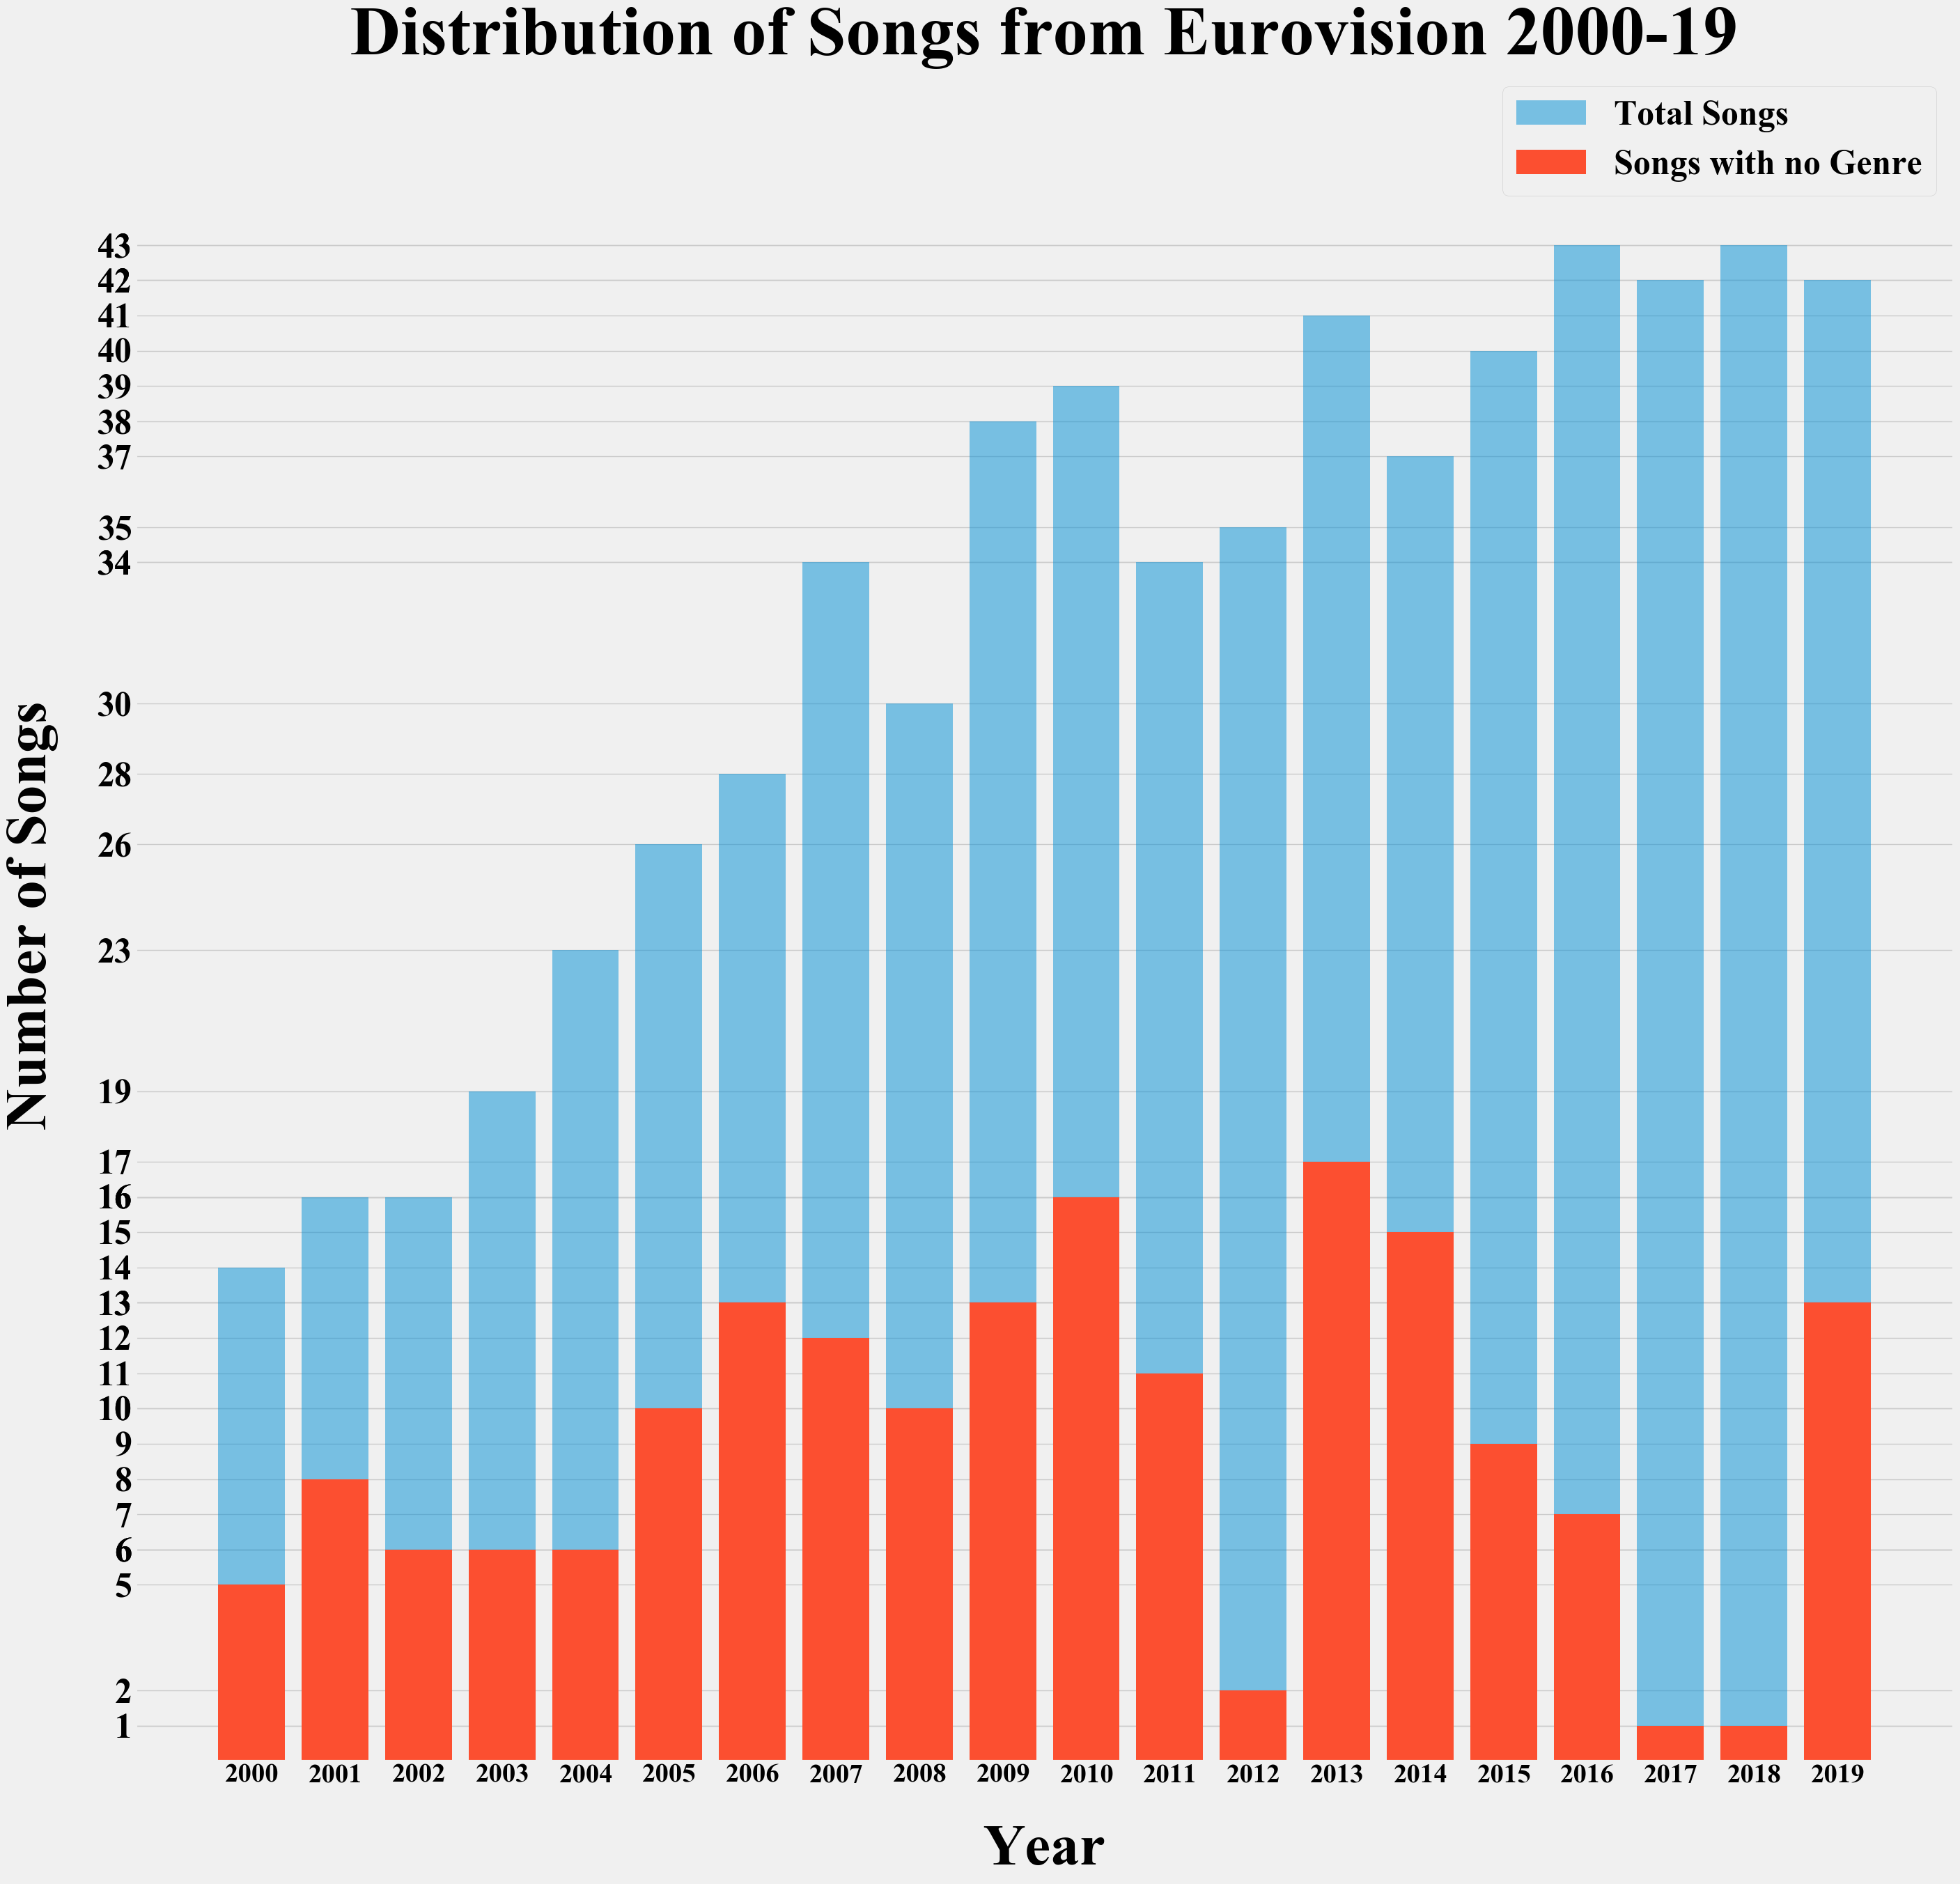
\includegraphics[width=\linewidth]{{final_plots/2_1_no_genres_00_19.png}}
  \centering
  \captionsetup{justification=centering}
  \caption{Frequency of Eurovision songs found in Spotify per
    year, from 2000 - 2019} 
  \label{fig:no_genres_00_19}
\end{figure}

From \Cref{fig:no_genres_00_19}

%\Cref{\cite{test}}
\cite{team_2020}
Hello there
\autocite{team_2020}

\begin{figure}[H]
  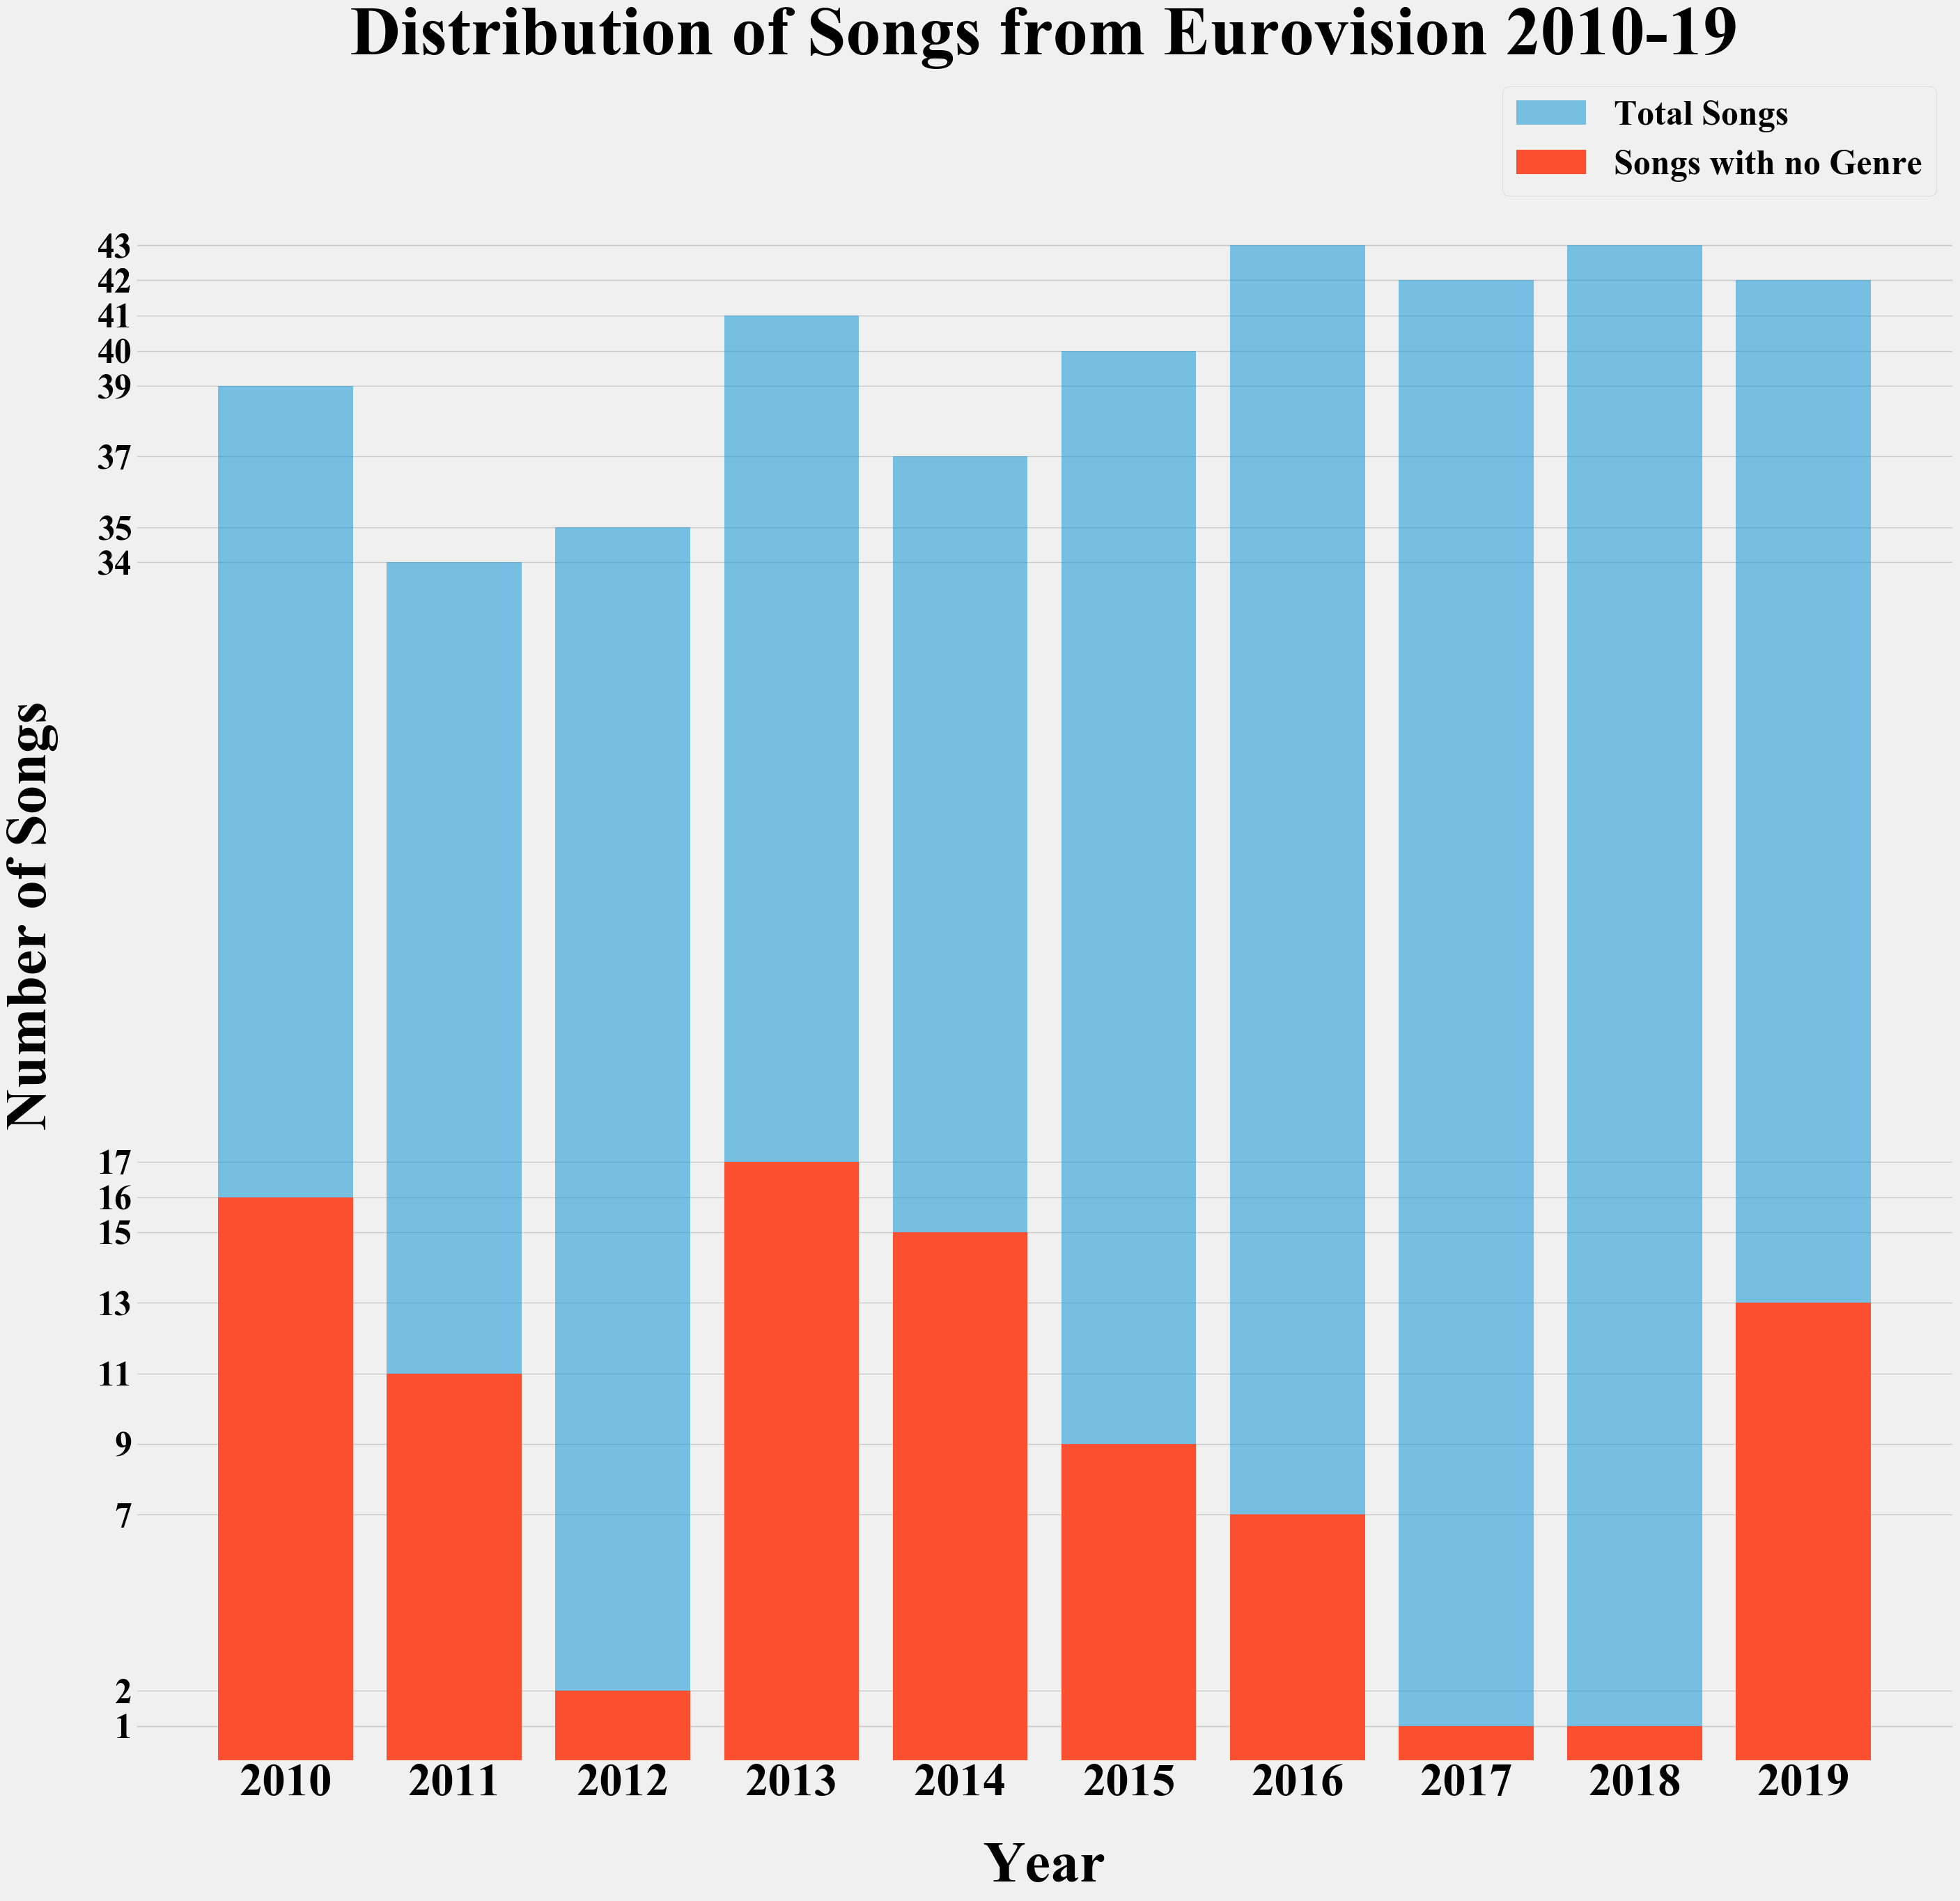
\includegraphics[width=\linewidth]{{final_plots/2_2_no_genres_10_19.png}}
  \centering
  \captionsetup{justification=centering}
  \caption{Frequency of Eurovision Songs Found in Spotify per Year
    Against Frequency of Songs per Year With No Genre, From 2010 –
    2019}
  \label{fig:no_genres_10_19}
\end{figure}

From \Cref{fig:no_genres_10_19}

\begin{figure}[H]
  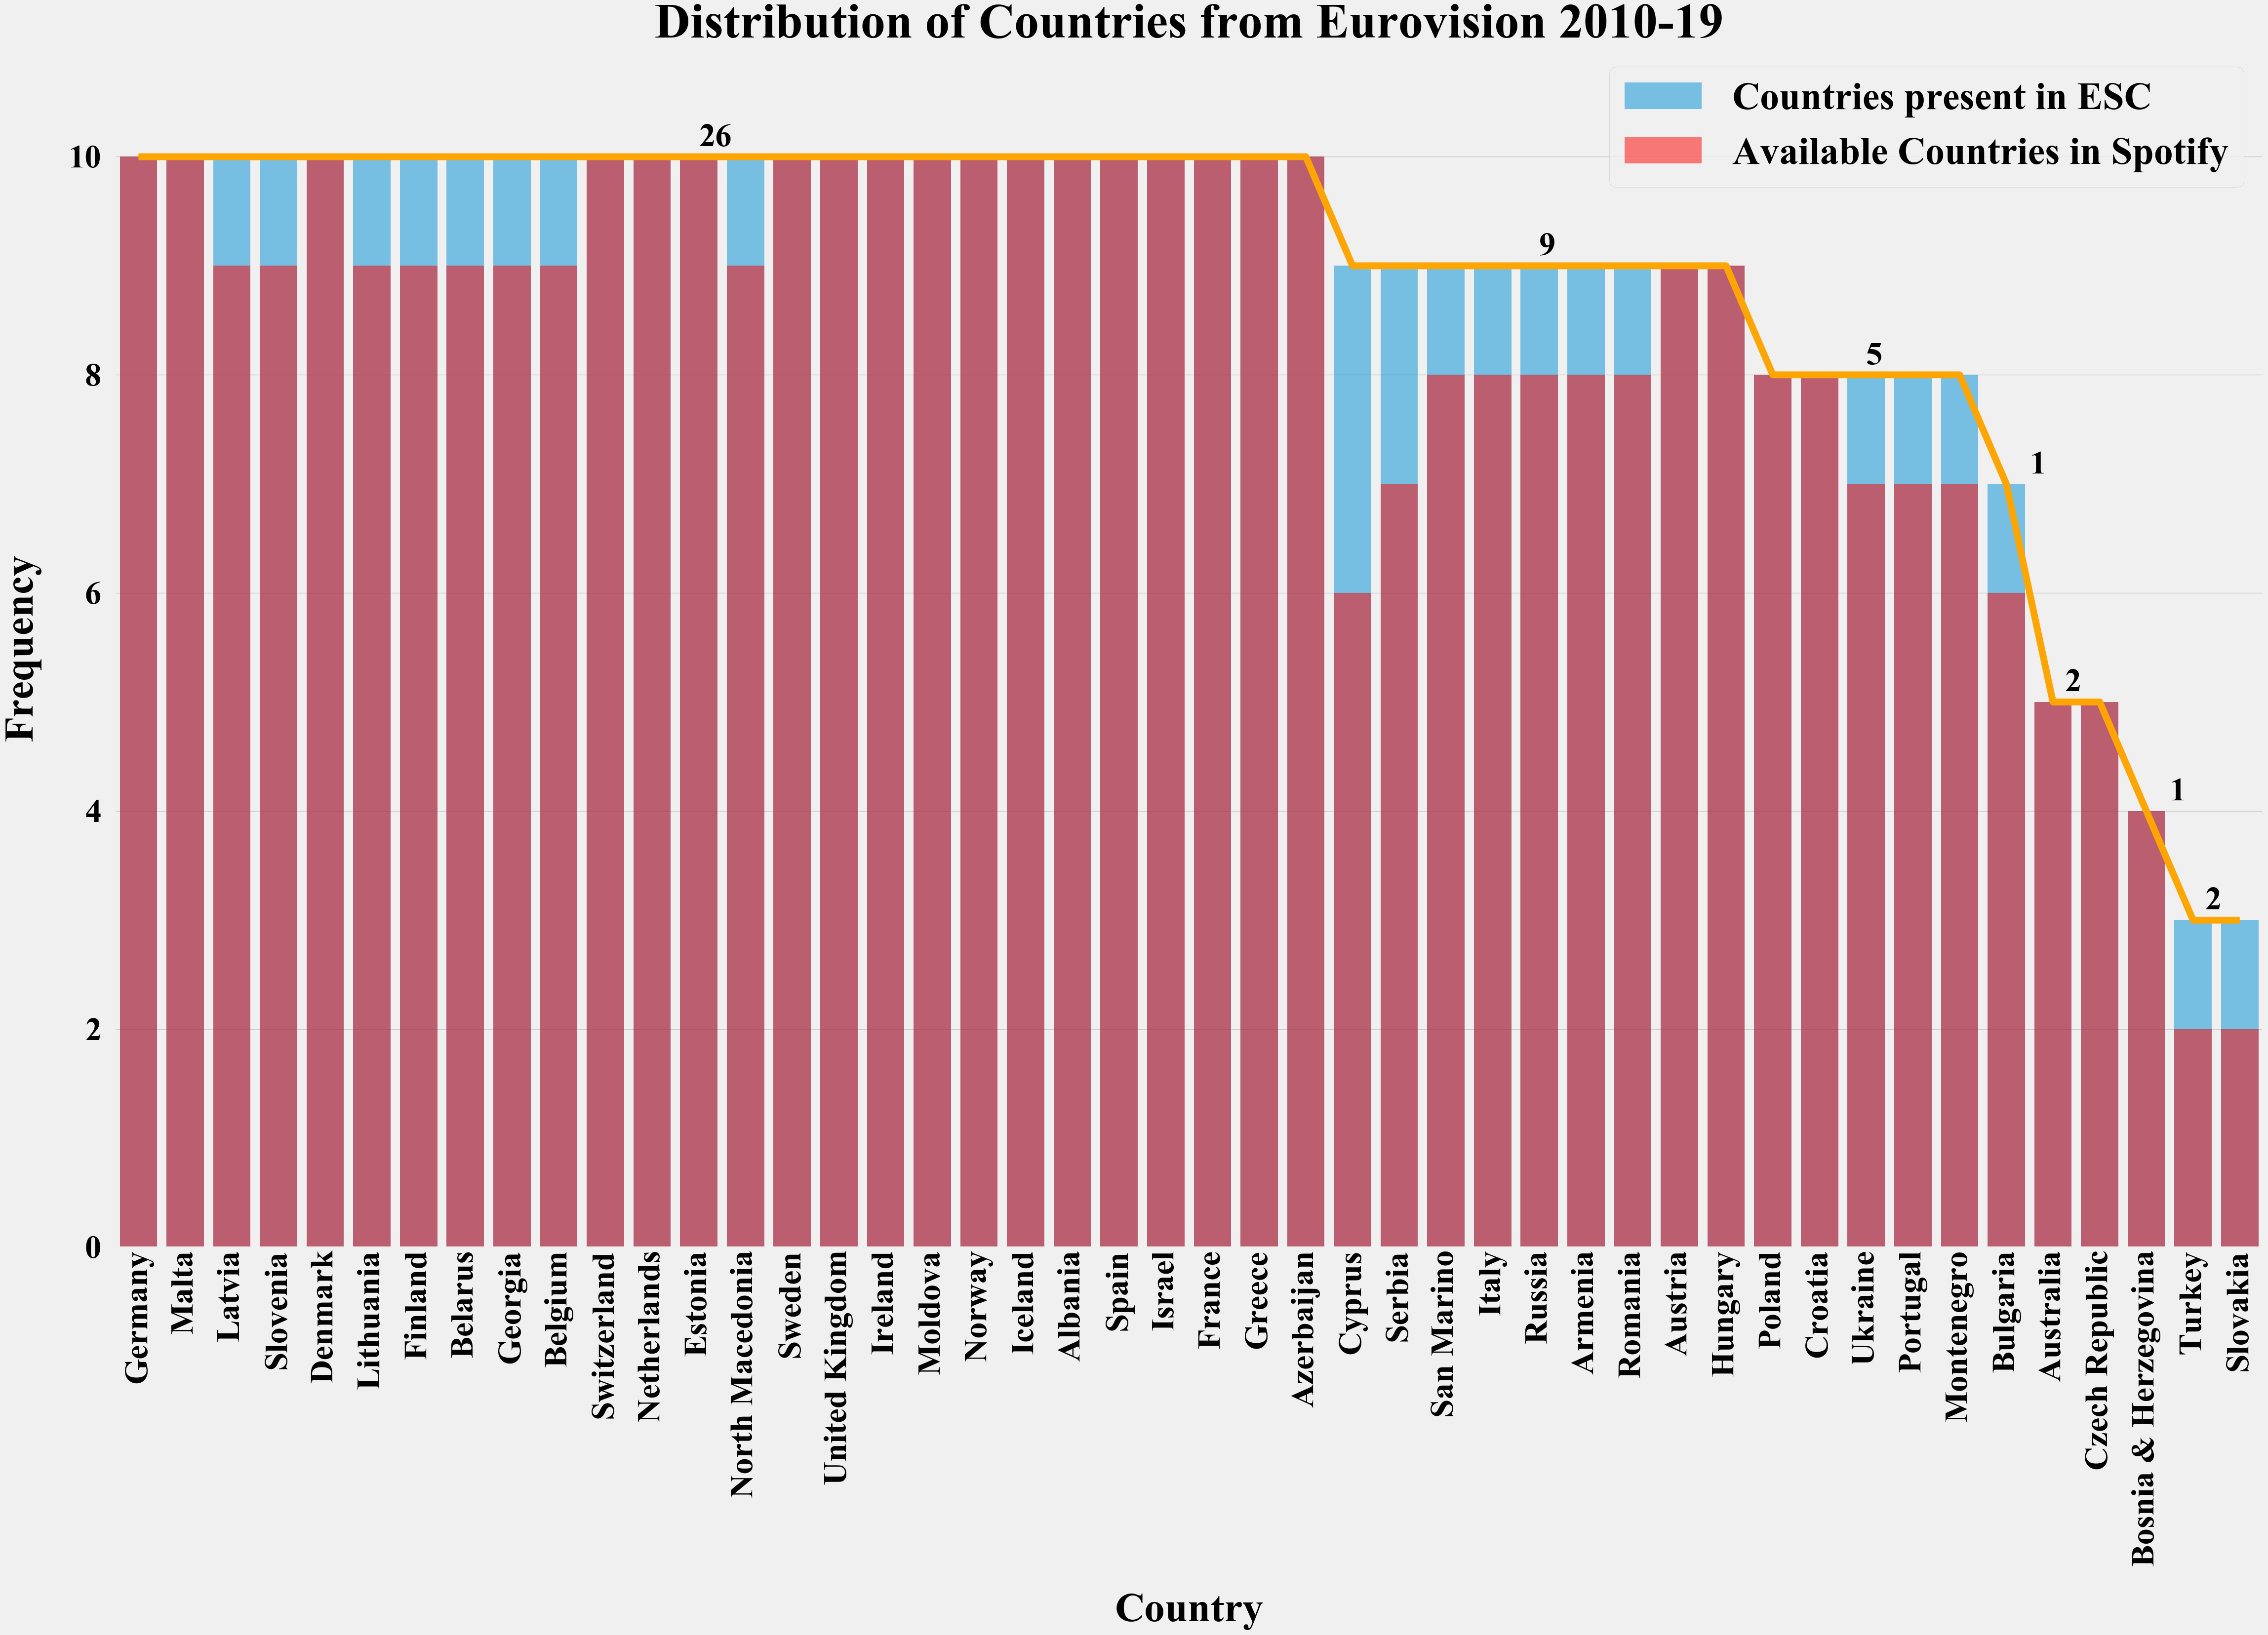
\includegraphics[width=\linewidth]{{final_plots/2_3_countries_10_19.png}}
  \centering
  \captionsetup{justification=centering}
  \caption{Frequency of Songs Found per Country Through Essentia and
    Spotify}
  \label{fig:countries_10_19}
\end{figure}

From \Cref{fig:countries_10_19}

% Defining Genre: Eurovision is Not One Genre
\newpage
\subsubsection{Defining Genre: Eurovision is Not One Genre}

\begin{figure}[H]
  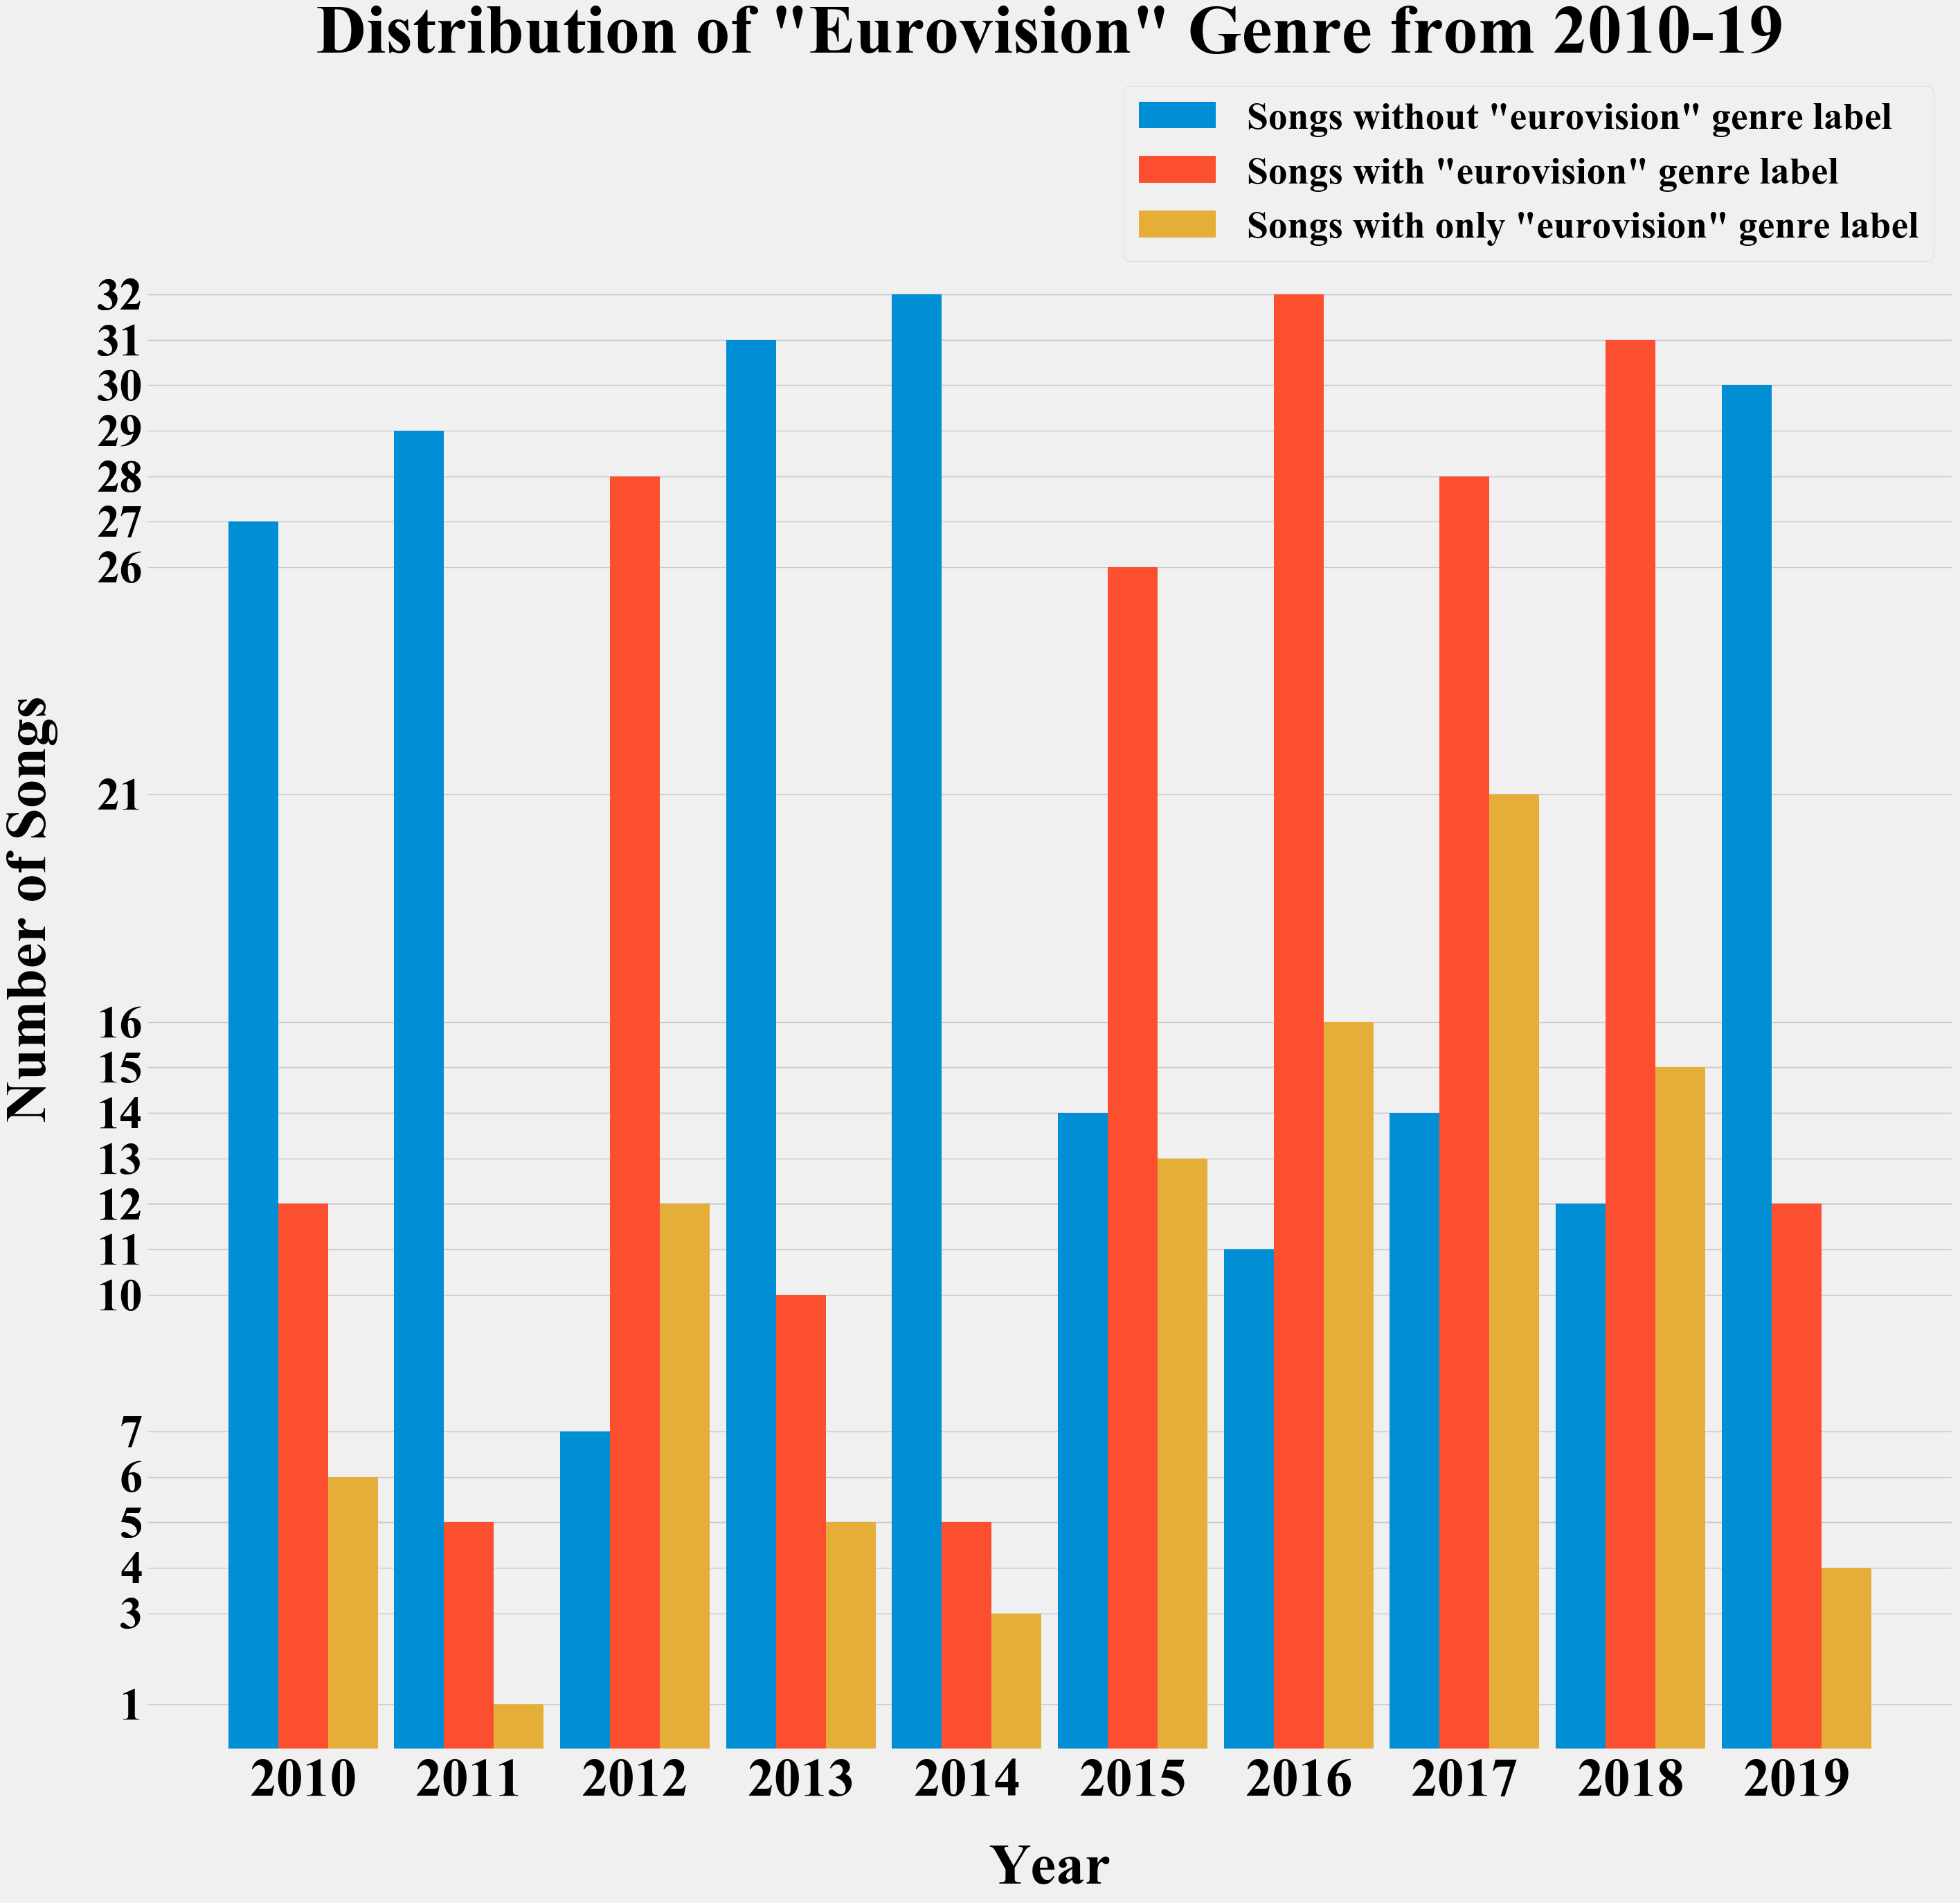
\includegraphics[width=\linewidth]{{final_plots/2_4_eurovision_10_19.png}}
  \centering
  \captionsetup{justification=centering}
  \caption{Analysis of “Eurovision” Genre From Spotify to Demonstrate
    Inconsistencies in a Dominant Genre} 
  \label{fig:eurovision_10_19}
\end{figure}

From \Cref{fig:eurovision_10_19}

\begin{figure}[H]
  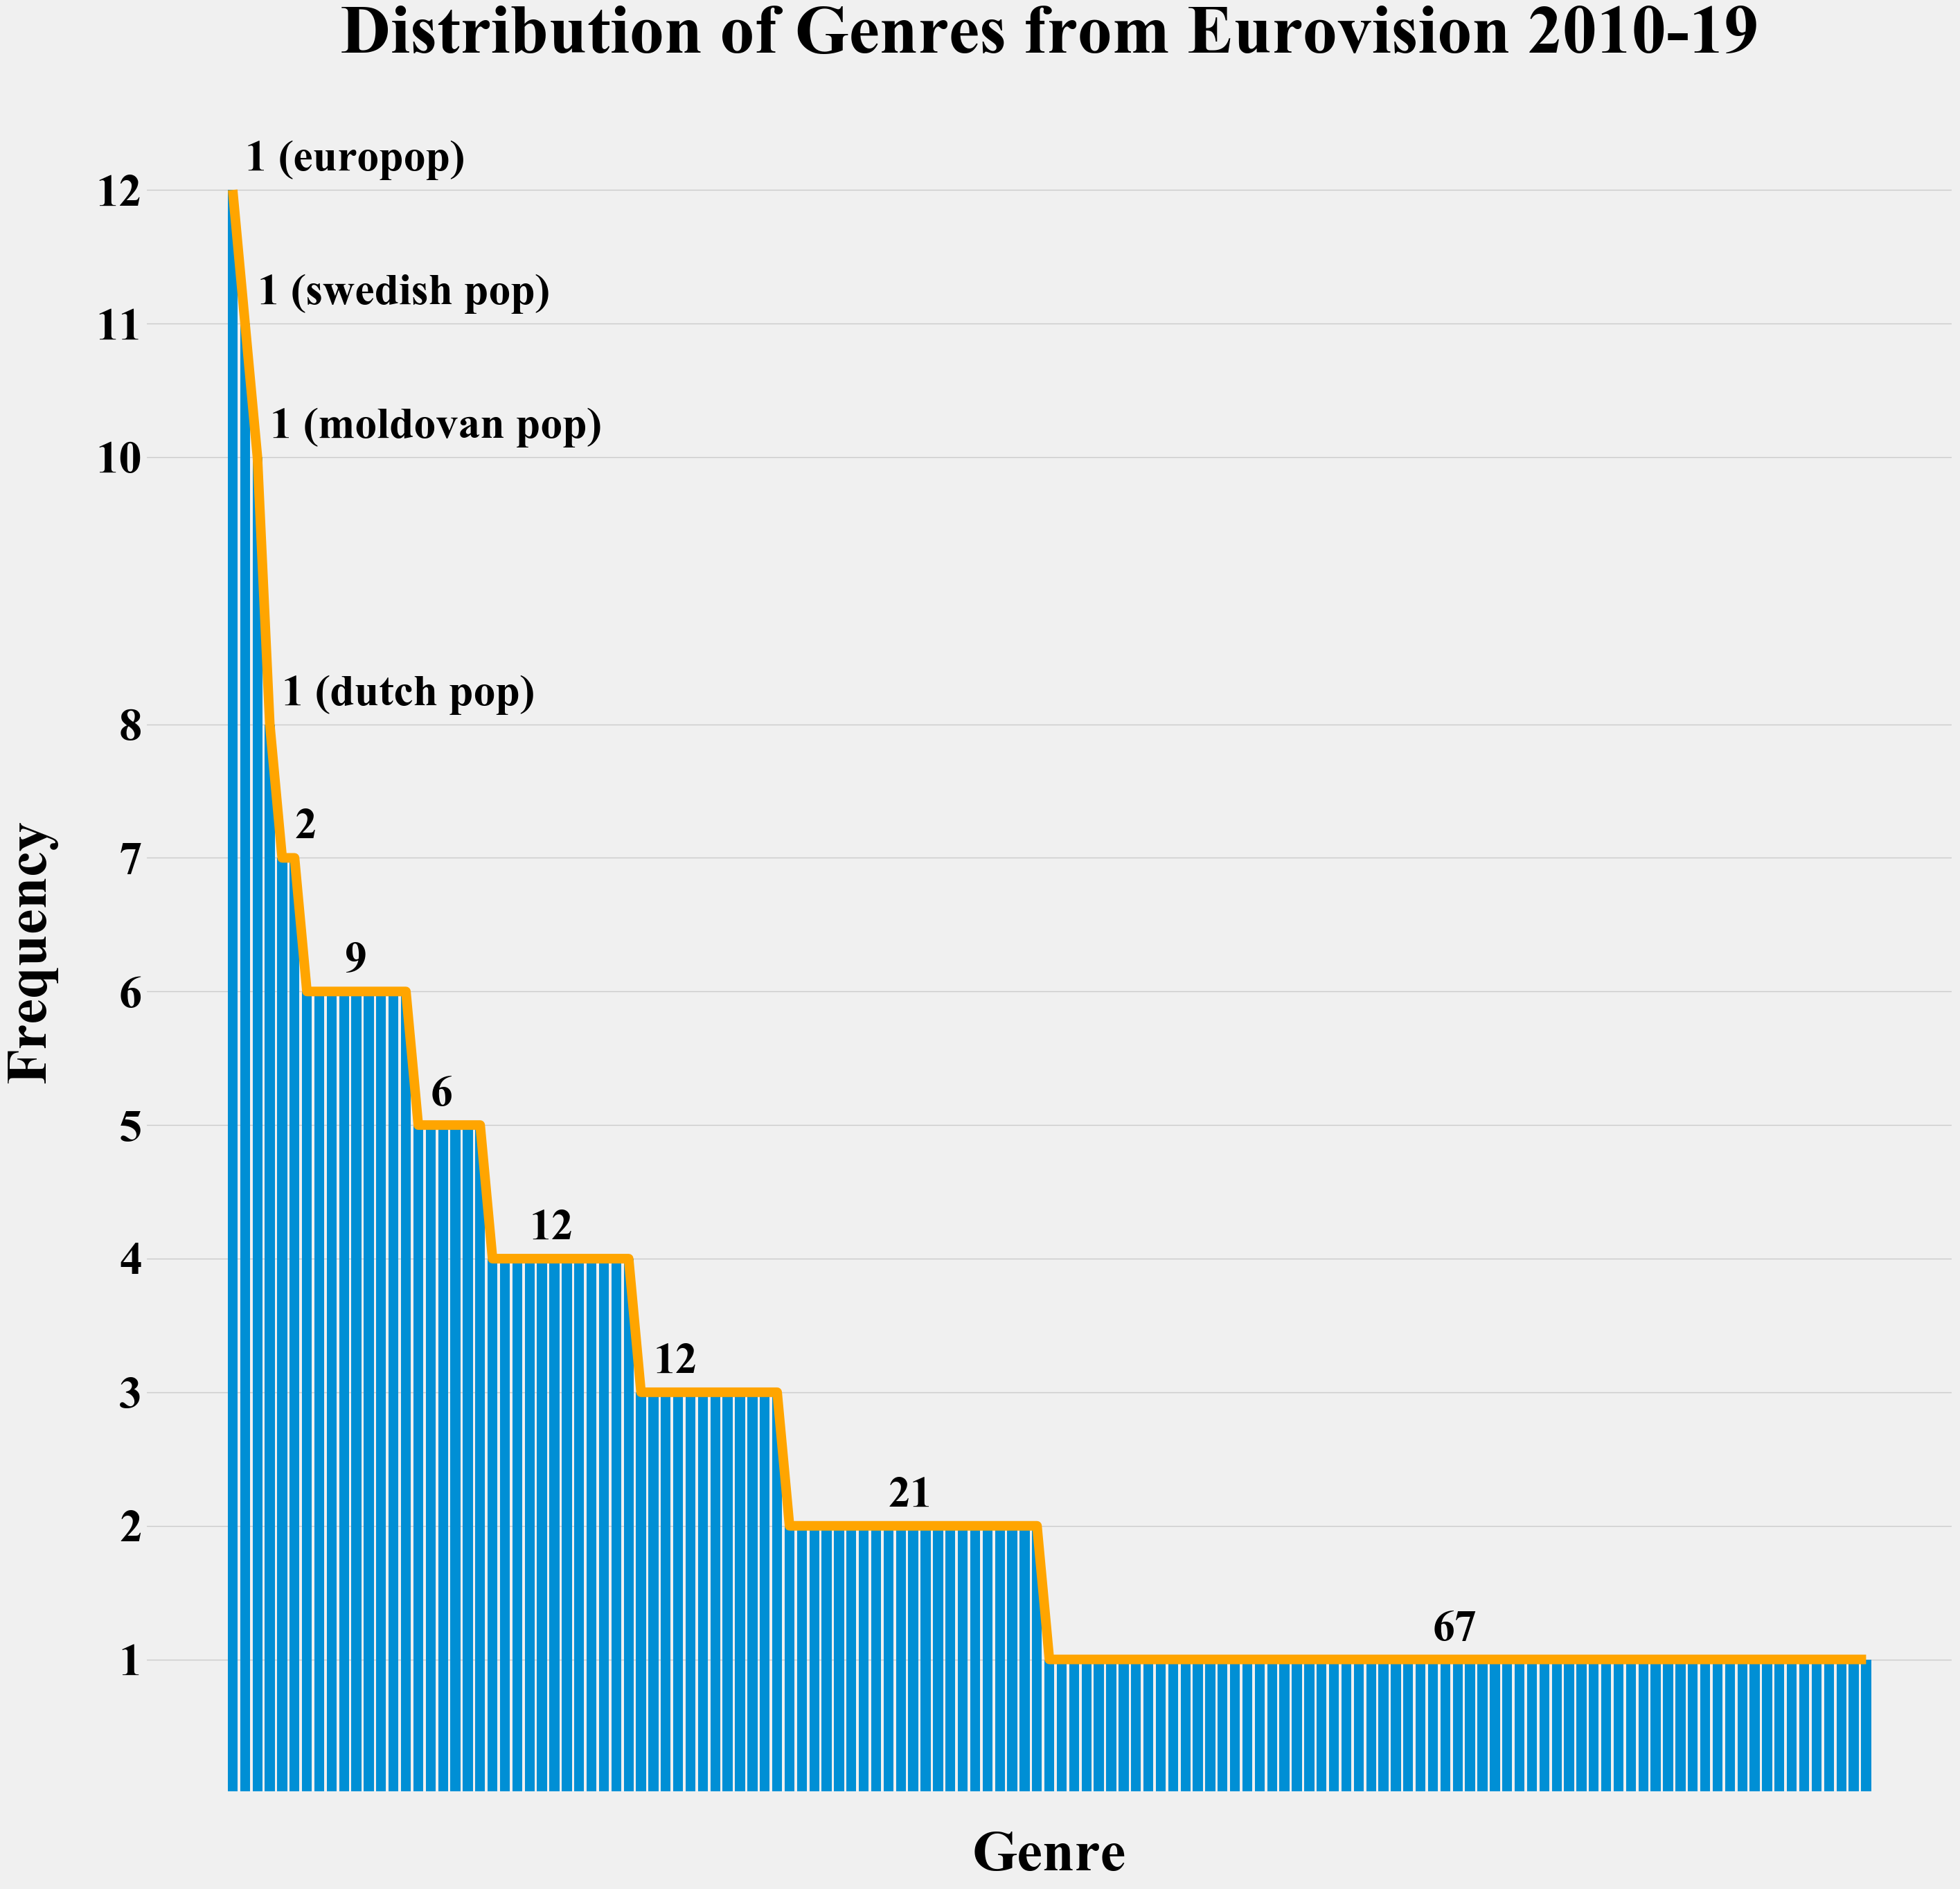
\includegraphics[width=\linewidth]{{final_plots/2_5_genres_10_19.png}}
  \centering
  \captionsetup{justification=centering}
  \caption{Distribution of Genres From Spotify to Explore the
    Diversity of Genres}
  \label{fig:genres_10_19}
\end{figure}

From \Cref{fig:genres_10_19}

\begin{figure}[H]
  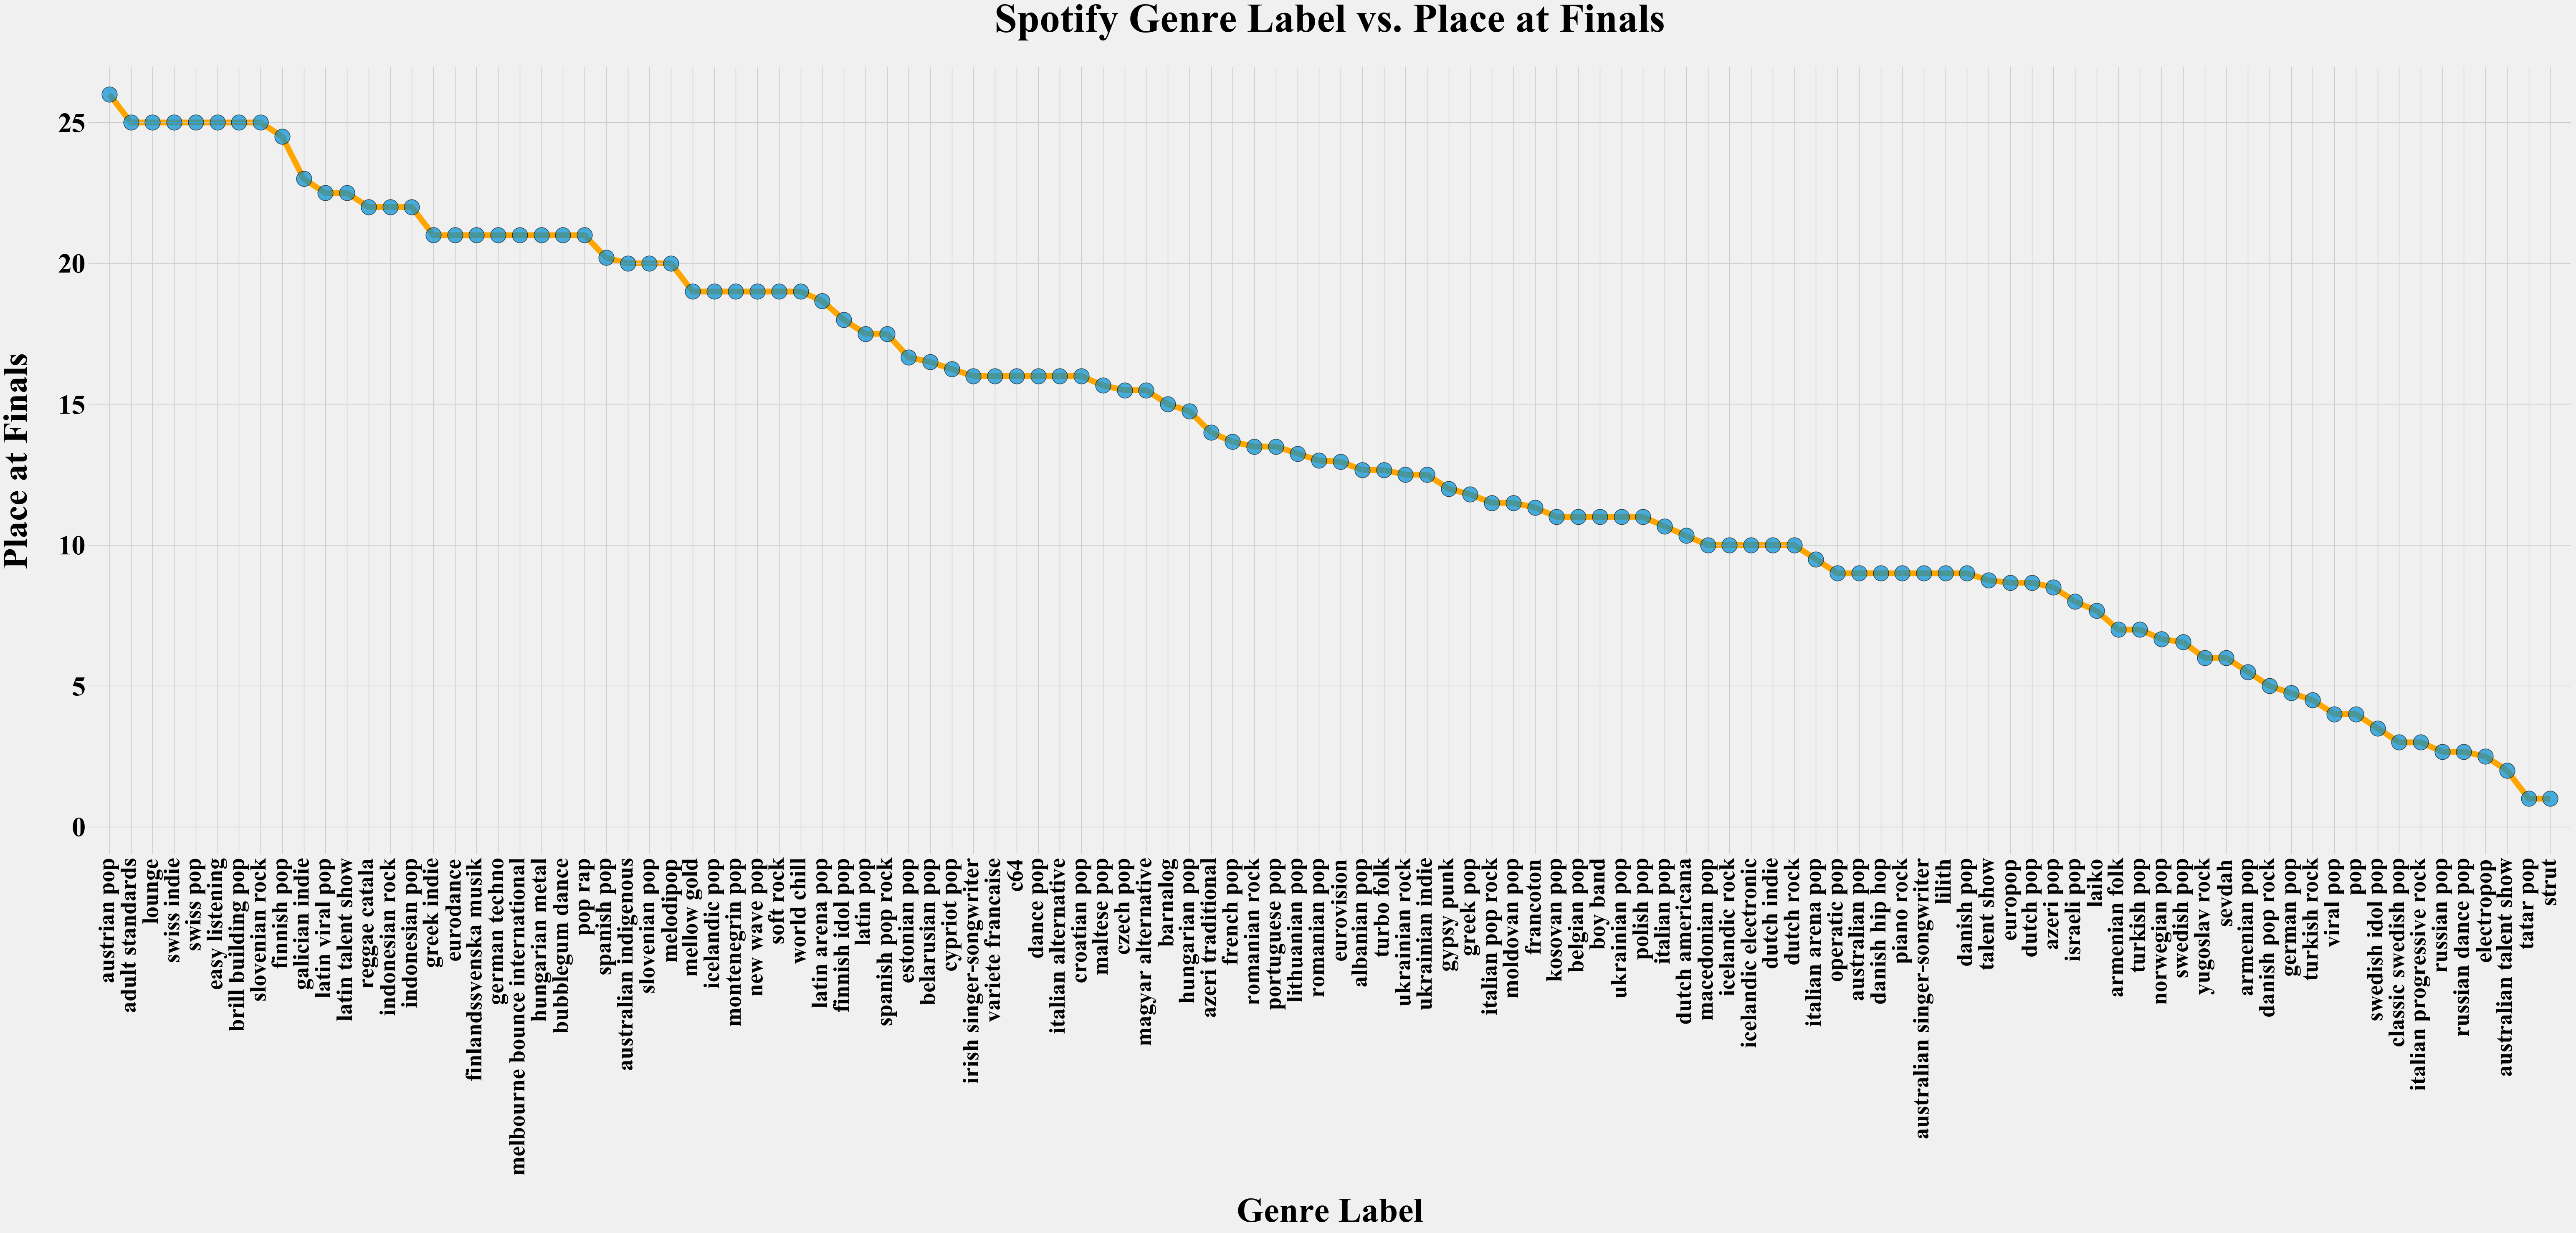
\includegraphics[width=\linewidth]{{final_plots/2_6_spotify_genre_place_final_sorted.png}}
  \centering
  \captionsetup{justification=centering}
  \caption{Plot of Genres From Spotify Against Average Final Place at
    the Eurovision to Describe Varying Appeal of Genres} 
  \label{fig:genre_place_final_sorted}
\end{figure}

From \Cref{fig:genre_place_final_sorted}

% Methods
\pagebreak
\section{Methods}
The ultimate goal of this research is to effectively illustrate the
relationship between a song’s intrinsic properties and its performance
at Eurovision. The strategy is to generate distinct genre
classifications, where each song is classified under a single
genre. Here, K-means is the chosen machine learning model for genre
classification. The clusters produced are treated as the genres since
the clusters are defined by musical features. To optimise the model, a
combination of a standard scaler, principal component analysis,
silhouette scoring metric, inertia, and distortion were applied
consecutively. The performances of the model both with and without
optimisation are compared against each other to evaluate the strength
of the entire pipeline.

\subsection{K-Means Clustering}
\subsection{Standard Scaler}
\subsection{Principal Component Analysis}
\subsection{Silhouette Score}
\subsection{Inertia and Distortion}

% Results
\newpage
\section{Results}
\renewcommand{\thefigure}{\thesection-\arabic{figure}}
\setcounter{figure}{0}

\begin{figure}[H]
  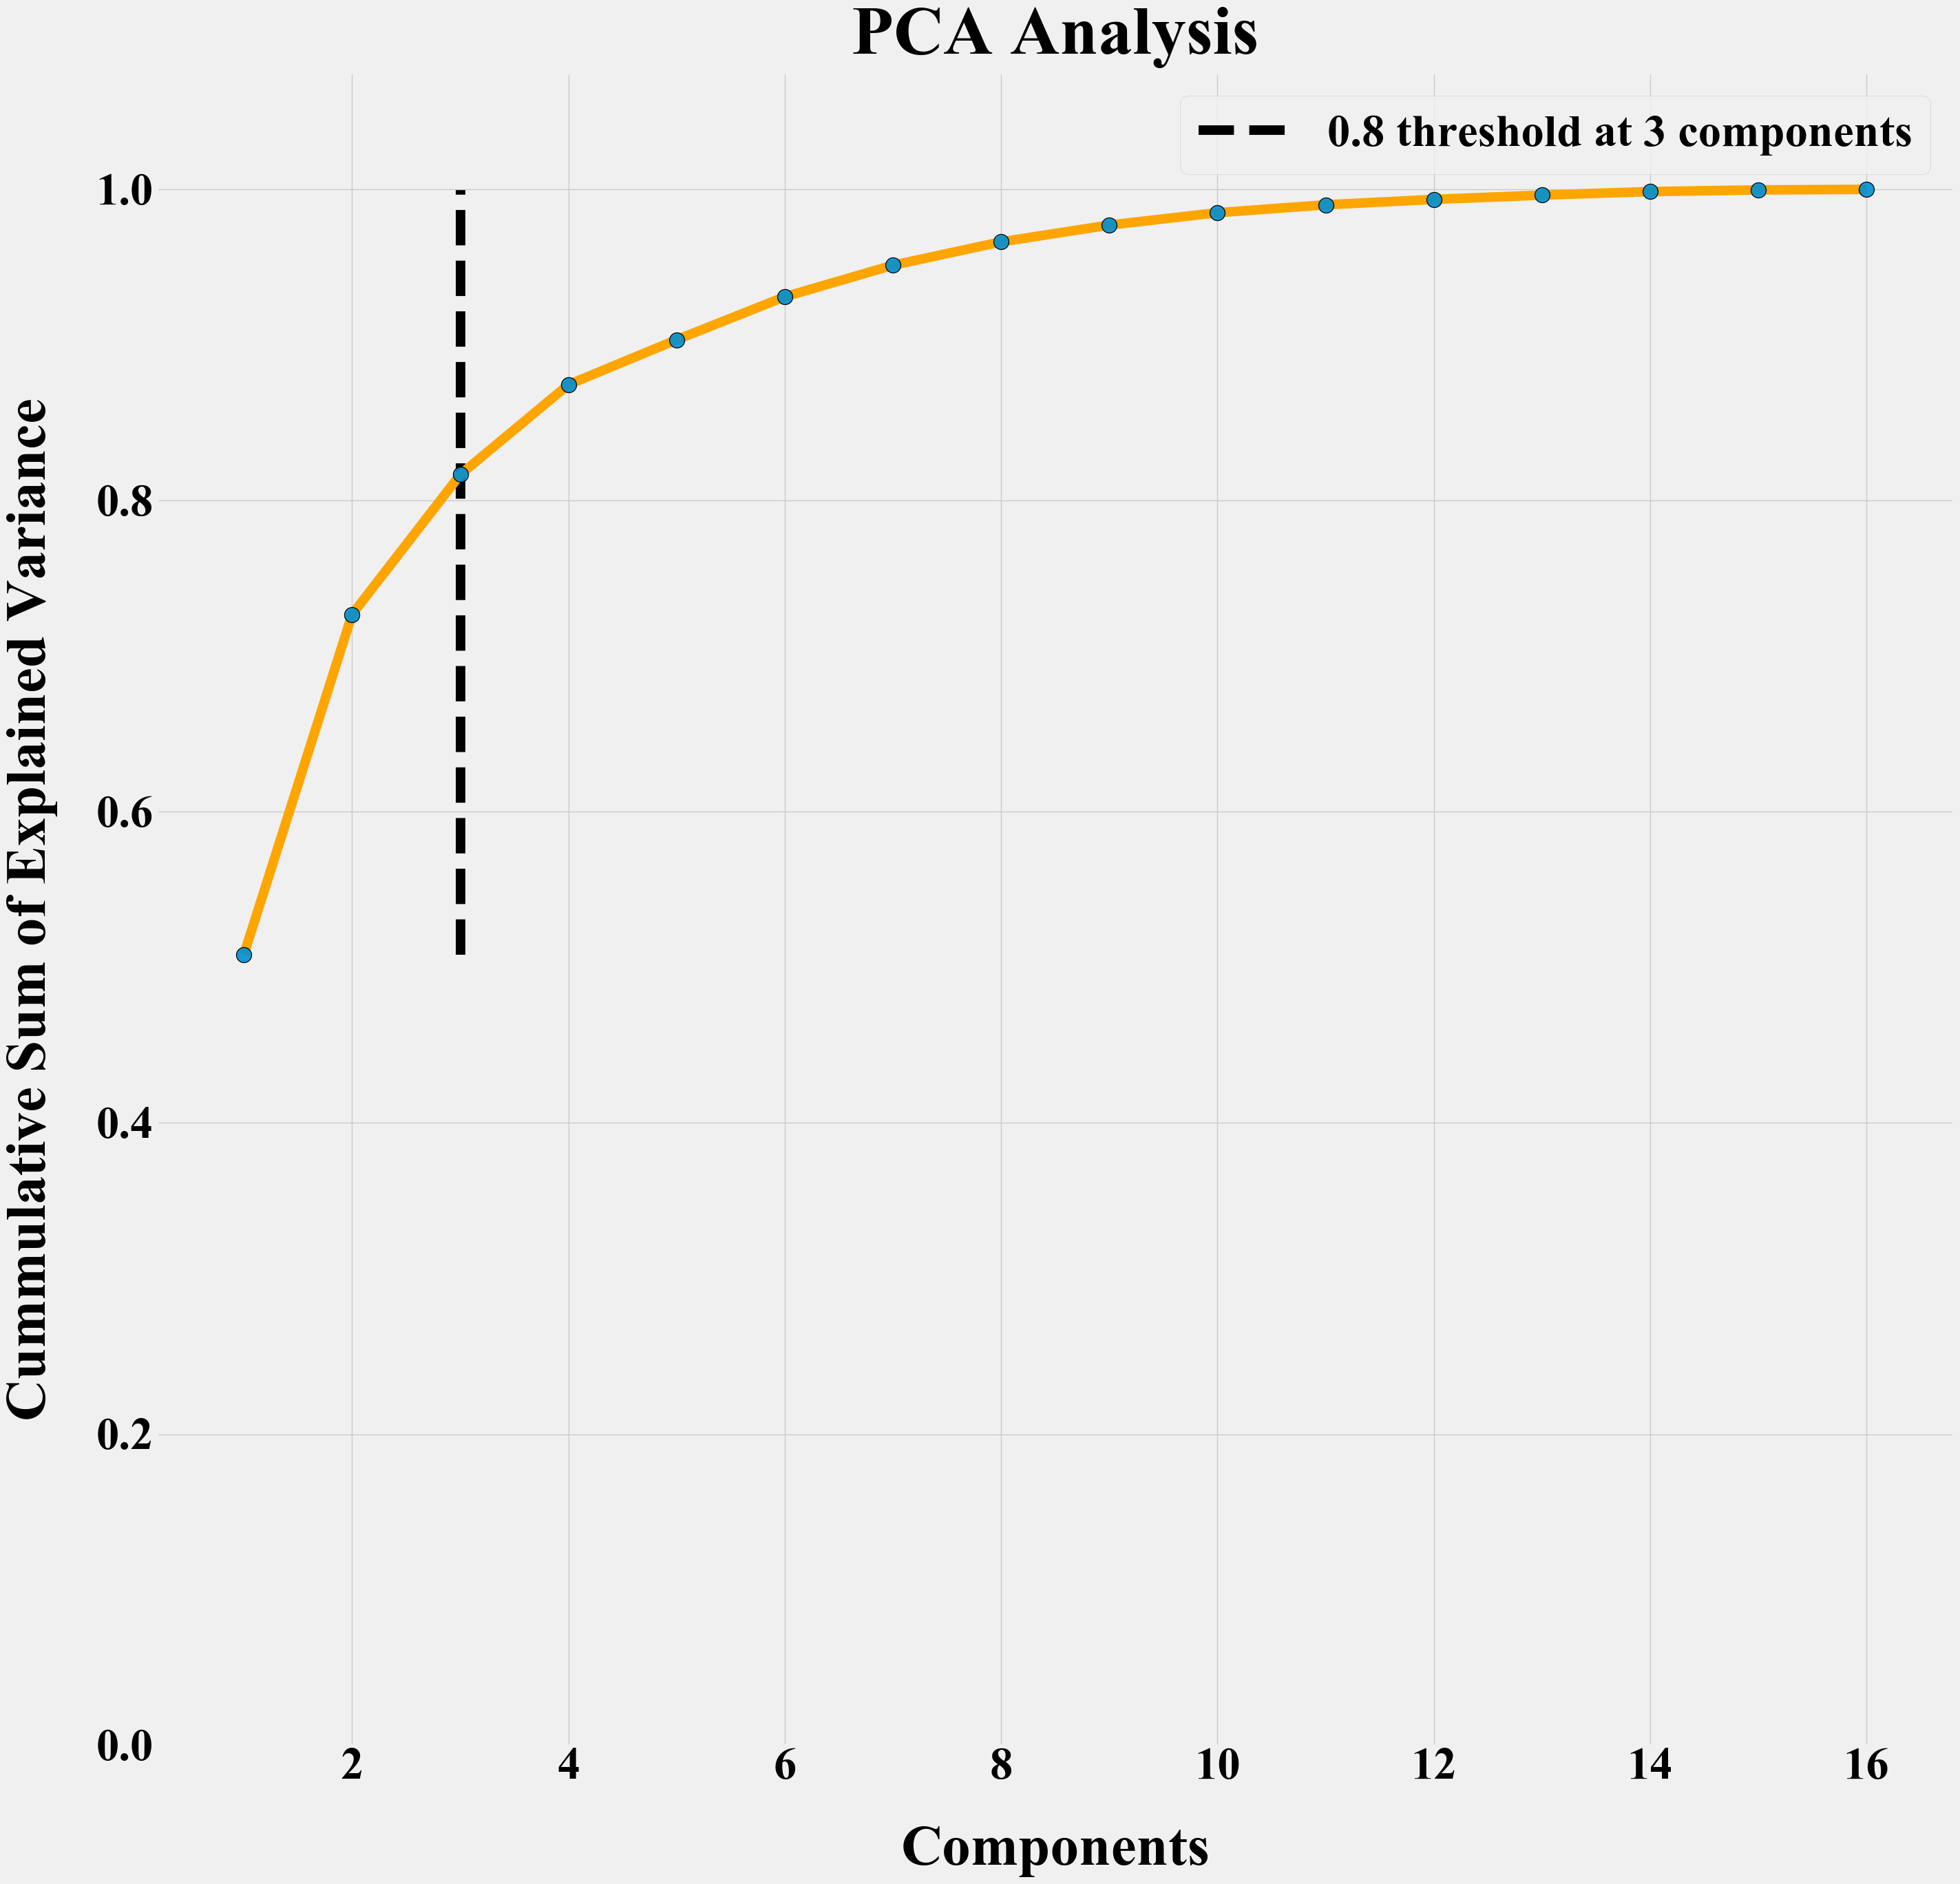
\includegraphics[width=\linewidth]{{final_plots/4_1_pca_evr_cumsum.png}}
  \centering
  \captionsetup{justification=centering}
  \caption{Explained Variance of PCA Scores Against the Number of Components Specified} 
  \label{fig:pca_evr_cumsum}
\end{figure}

From \Cref{fig:pca_evr_cumsum}

\begin{figure}[H]
  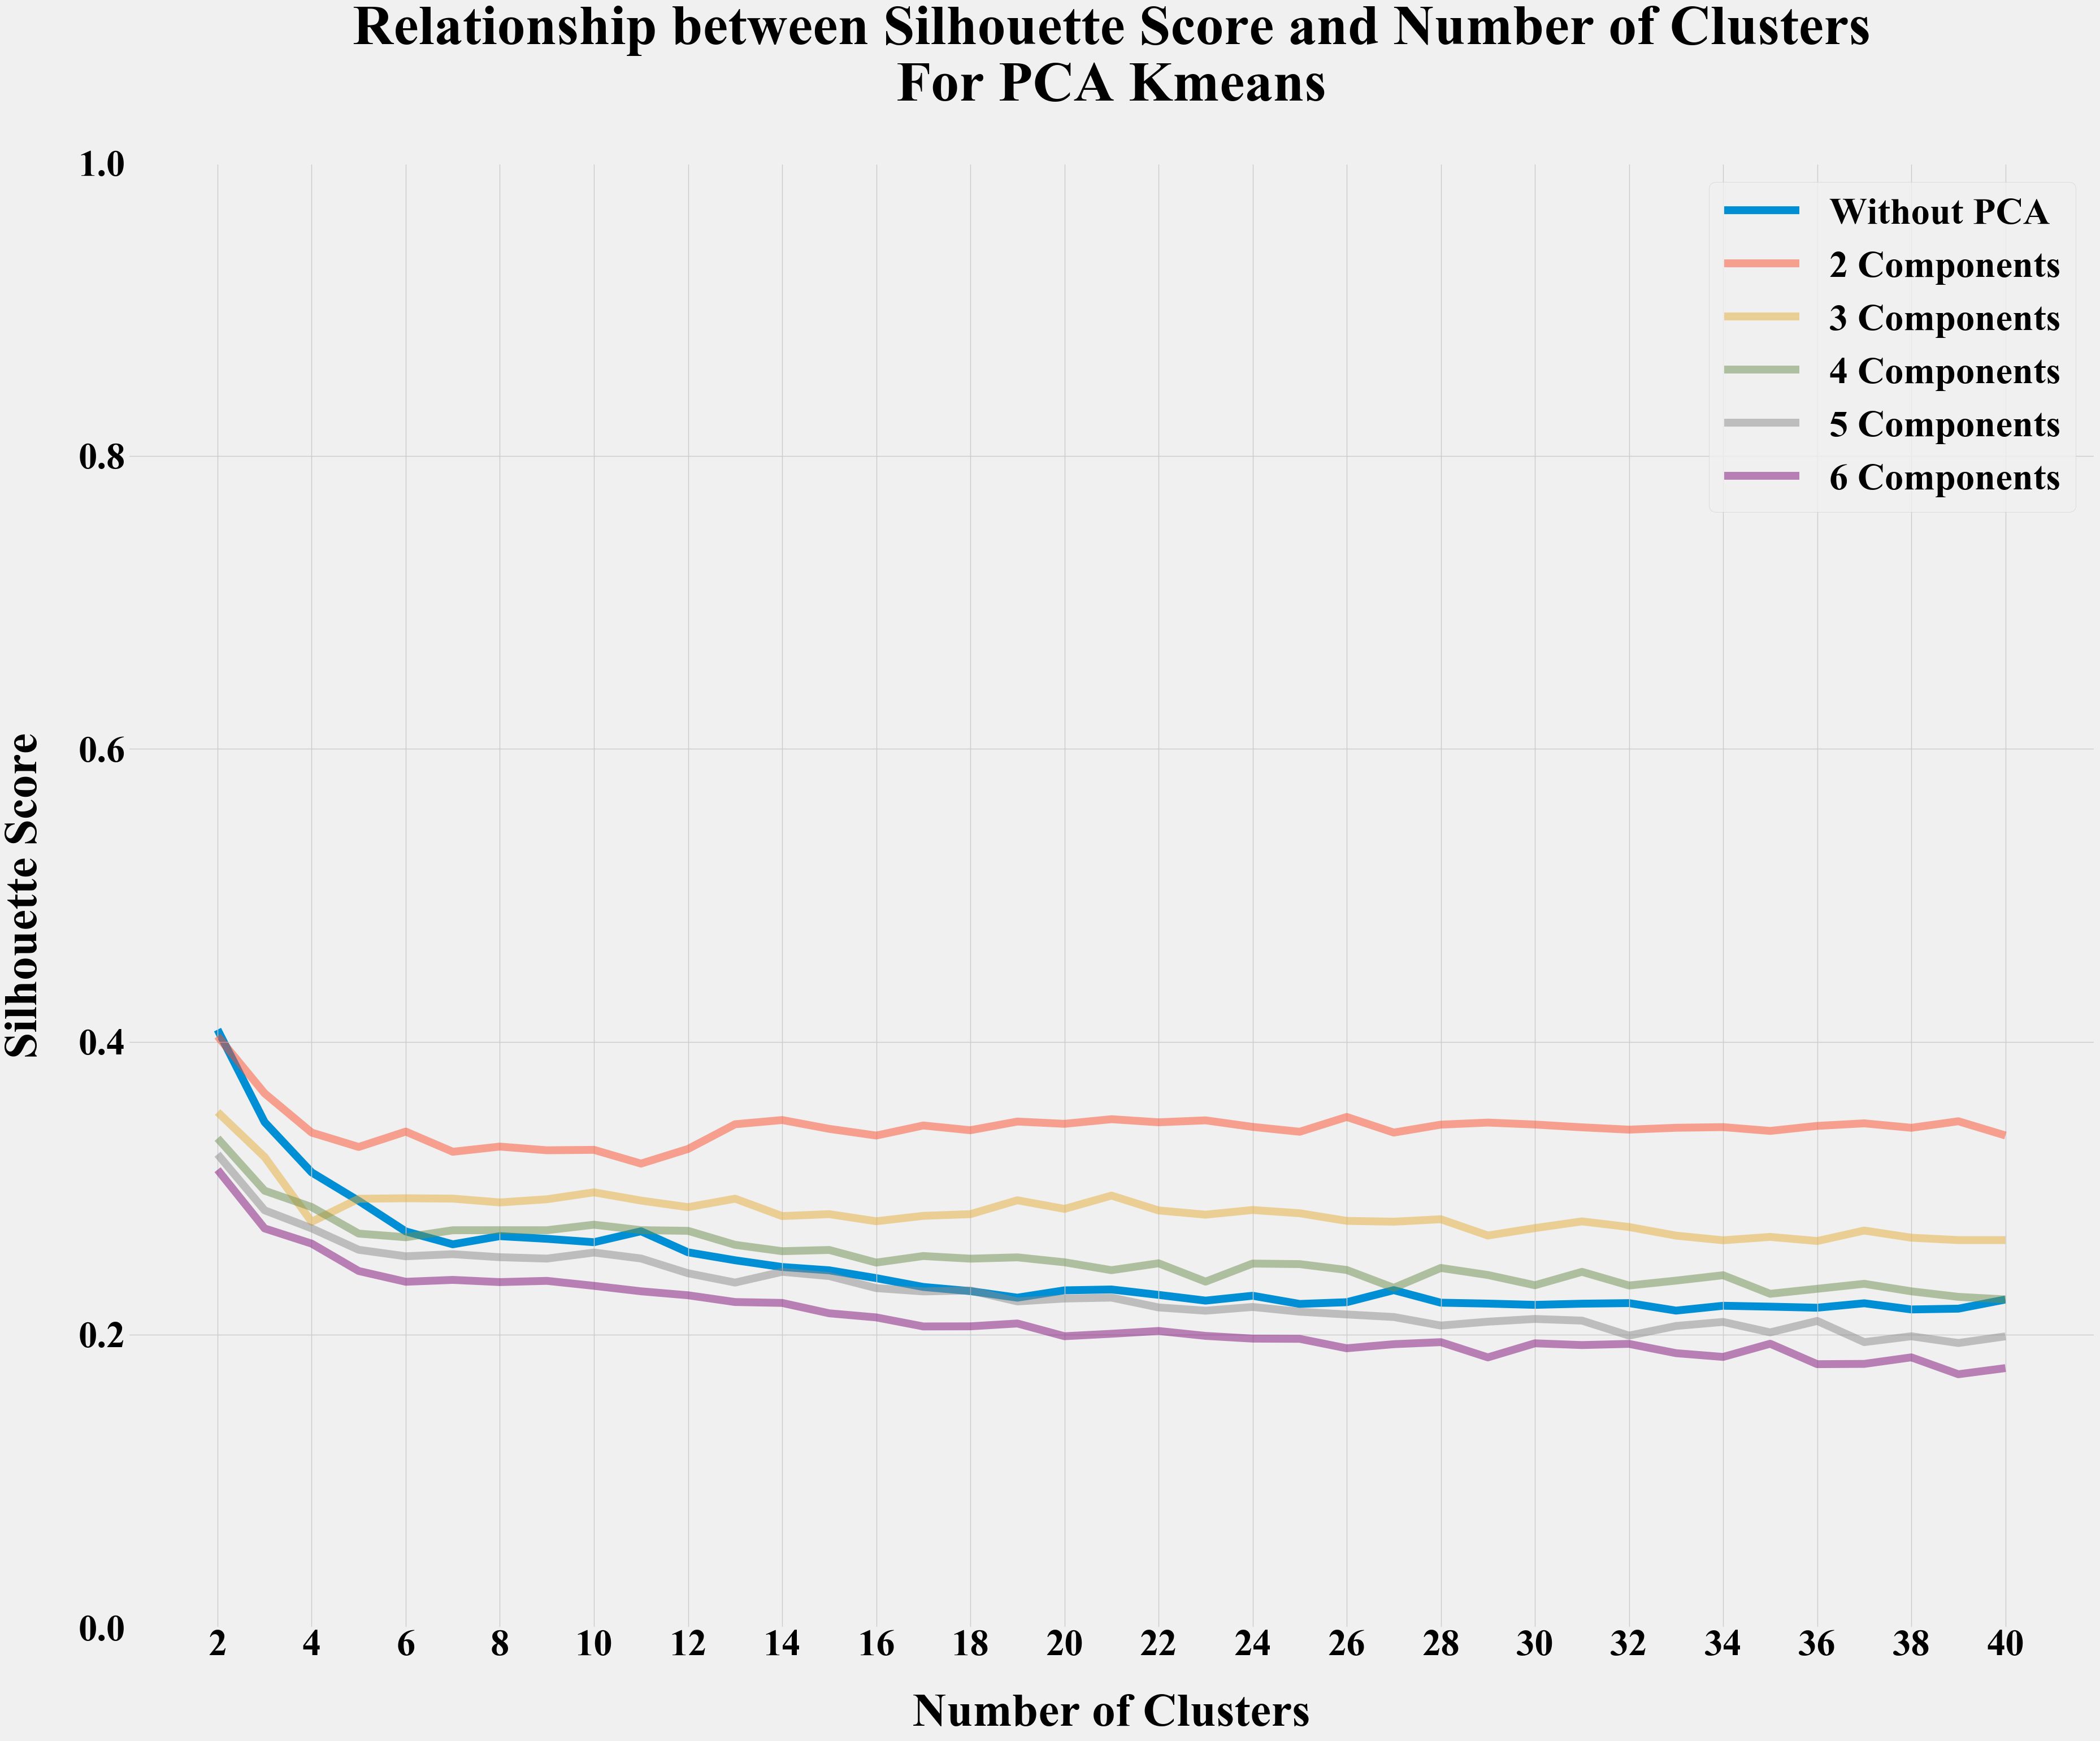
\includegraphics[width=\linewidth]{{final_plots/4_2_sil_scores_multi_pca_kmeans.png}}
  \centering
  \captionsetup{justification=centering}
  \caption{Average Silhouette Score to Distinguish Varying Principal Components} 
  \label{fig:sil_scores_multi_pca_kmeans}
\end{figure}

From \Cref{fig:sil_scores_multi_pca_kmeans}

\begin{figure}[H]
  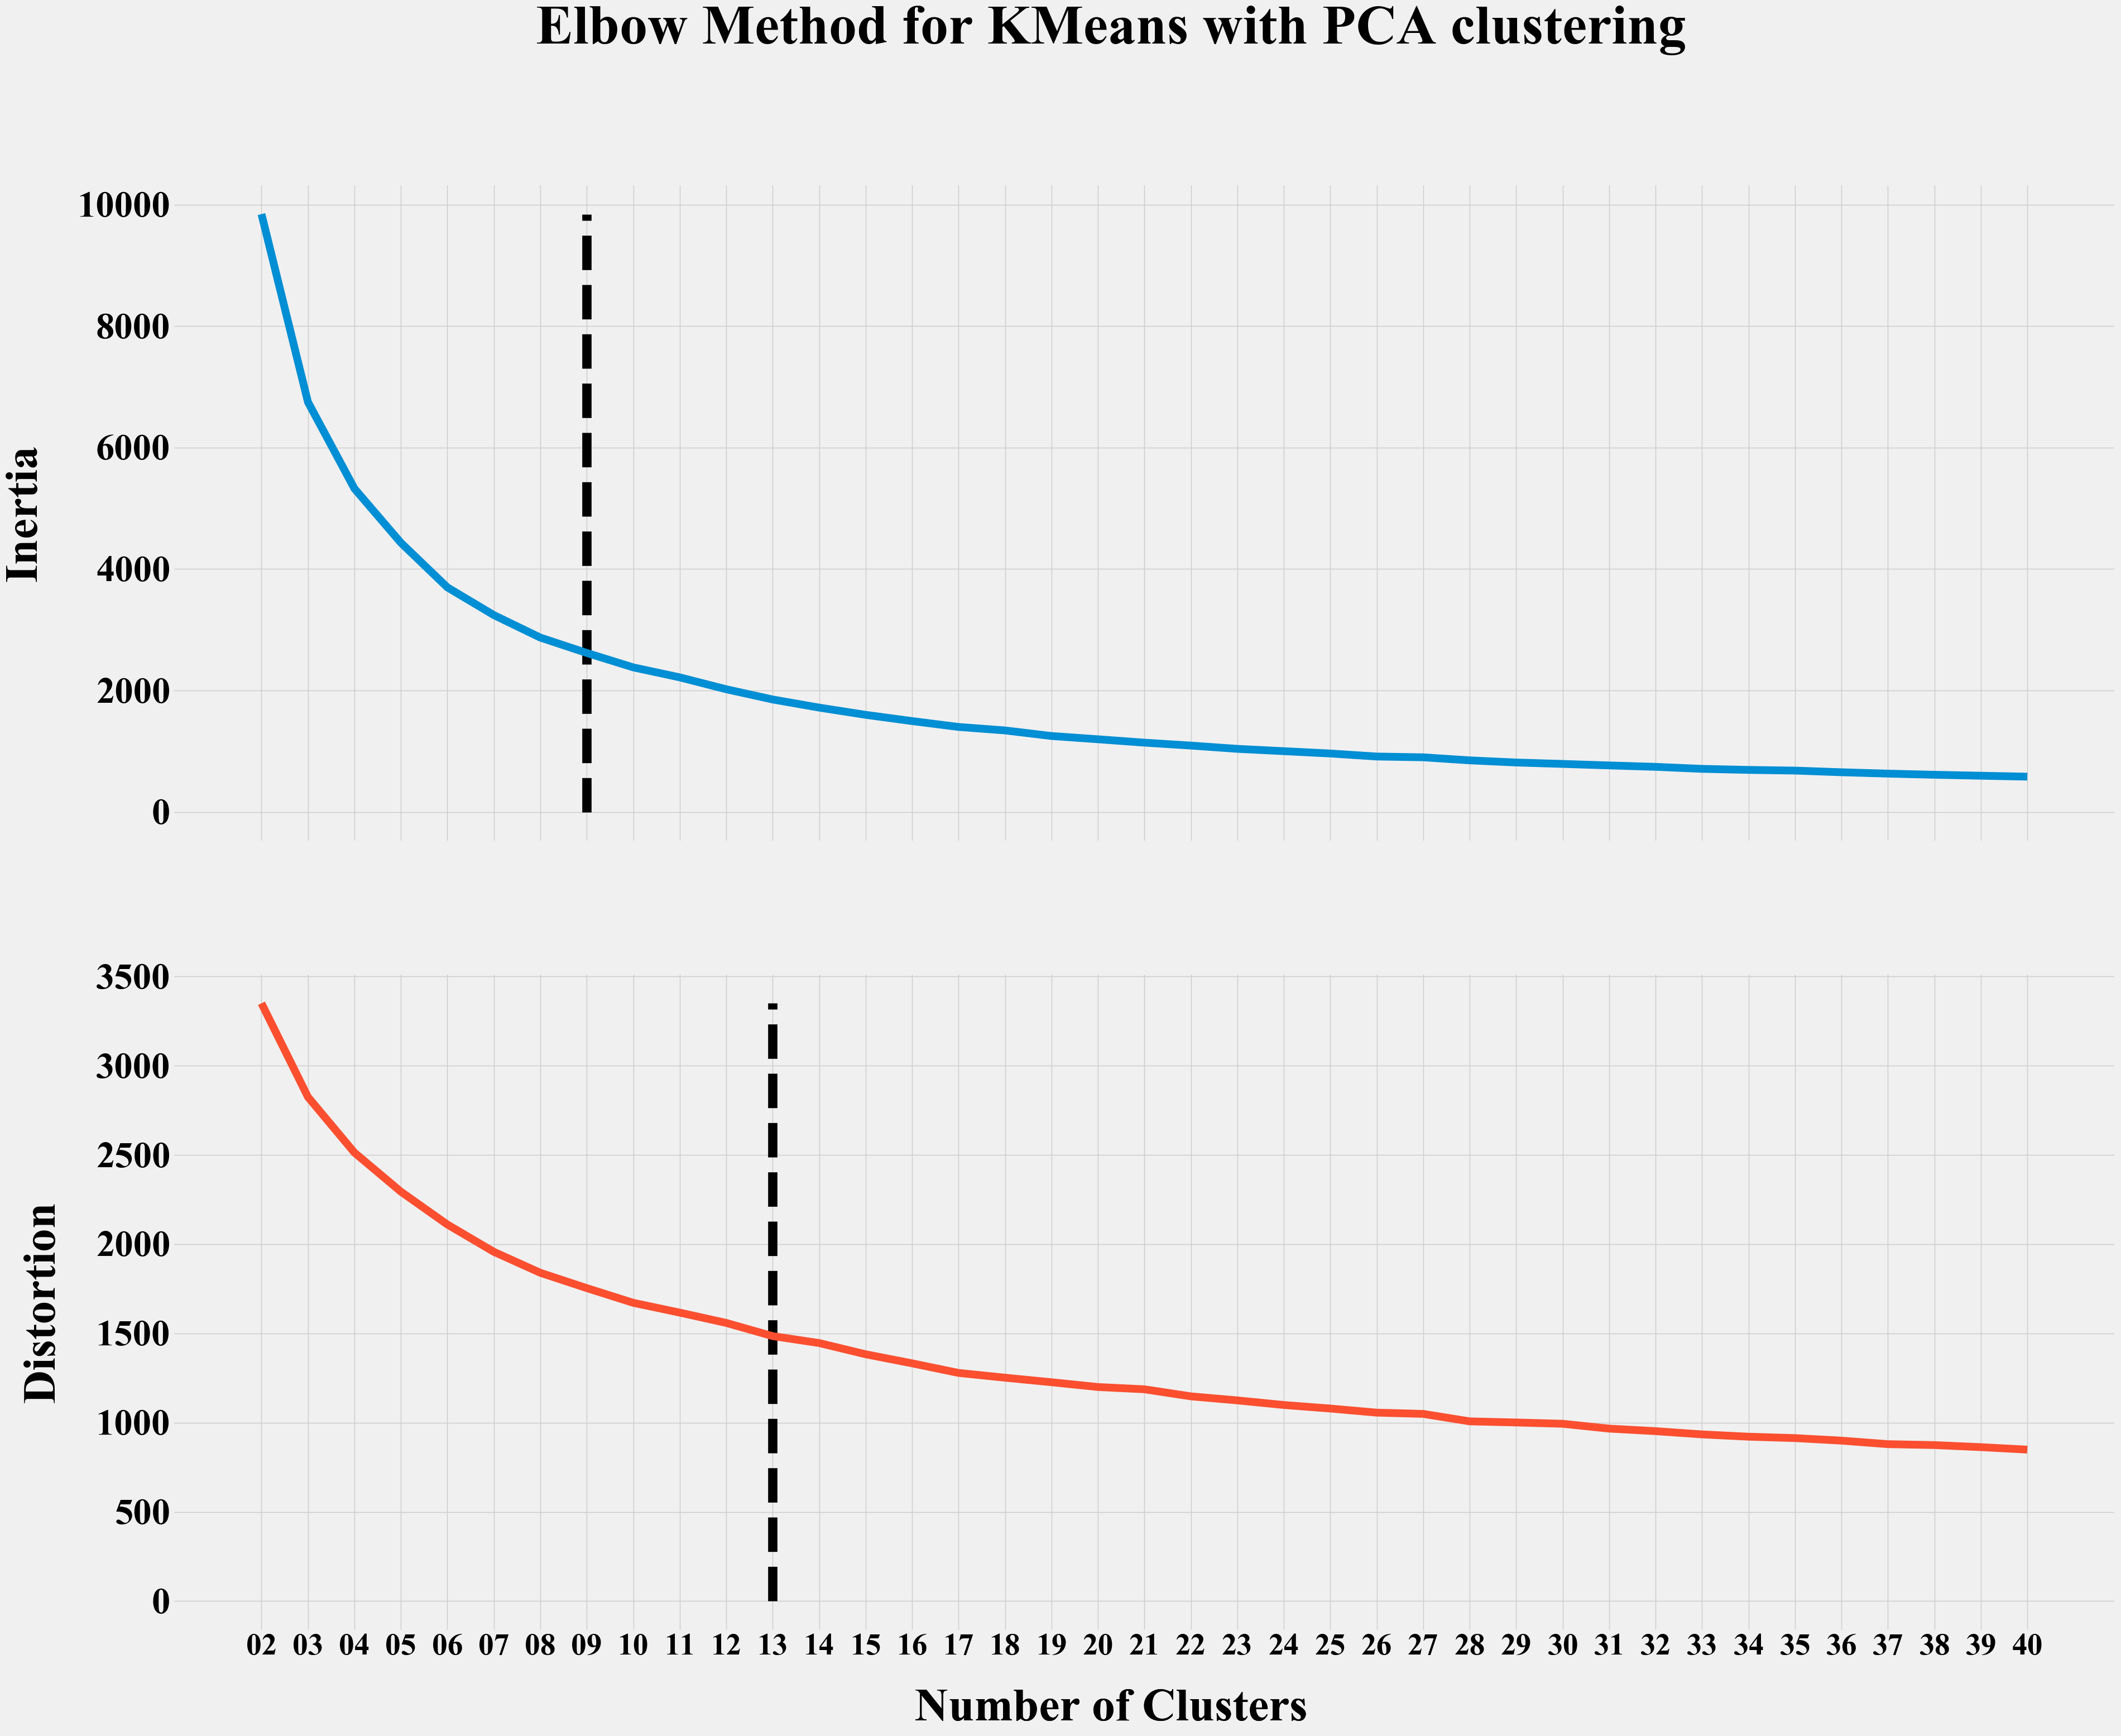
\includegraphics[width=\linewidth]{{final_plots/4_3_elbow_pca_kmeans.png}}
  \centering
  \captionsetup{justification=centering}
  \caption{Plots of Inertia and Distortion to Narrow Selection of Number of Clusters} 
  \label{fig:elbow_pca_kmeans}
\end{figure}

From \Cref{fig:elbow_pca_kmeans}

\begin{figure}[H]
  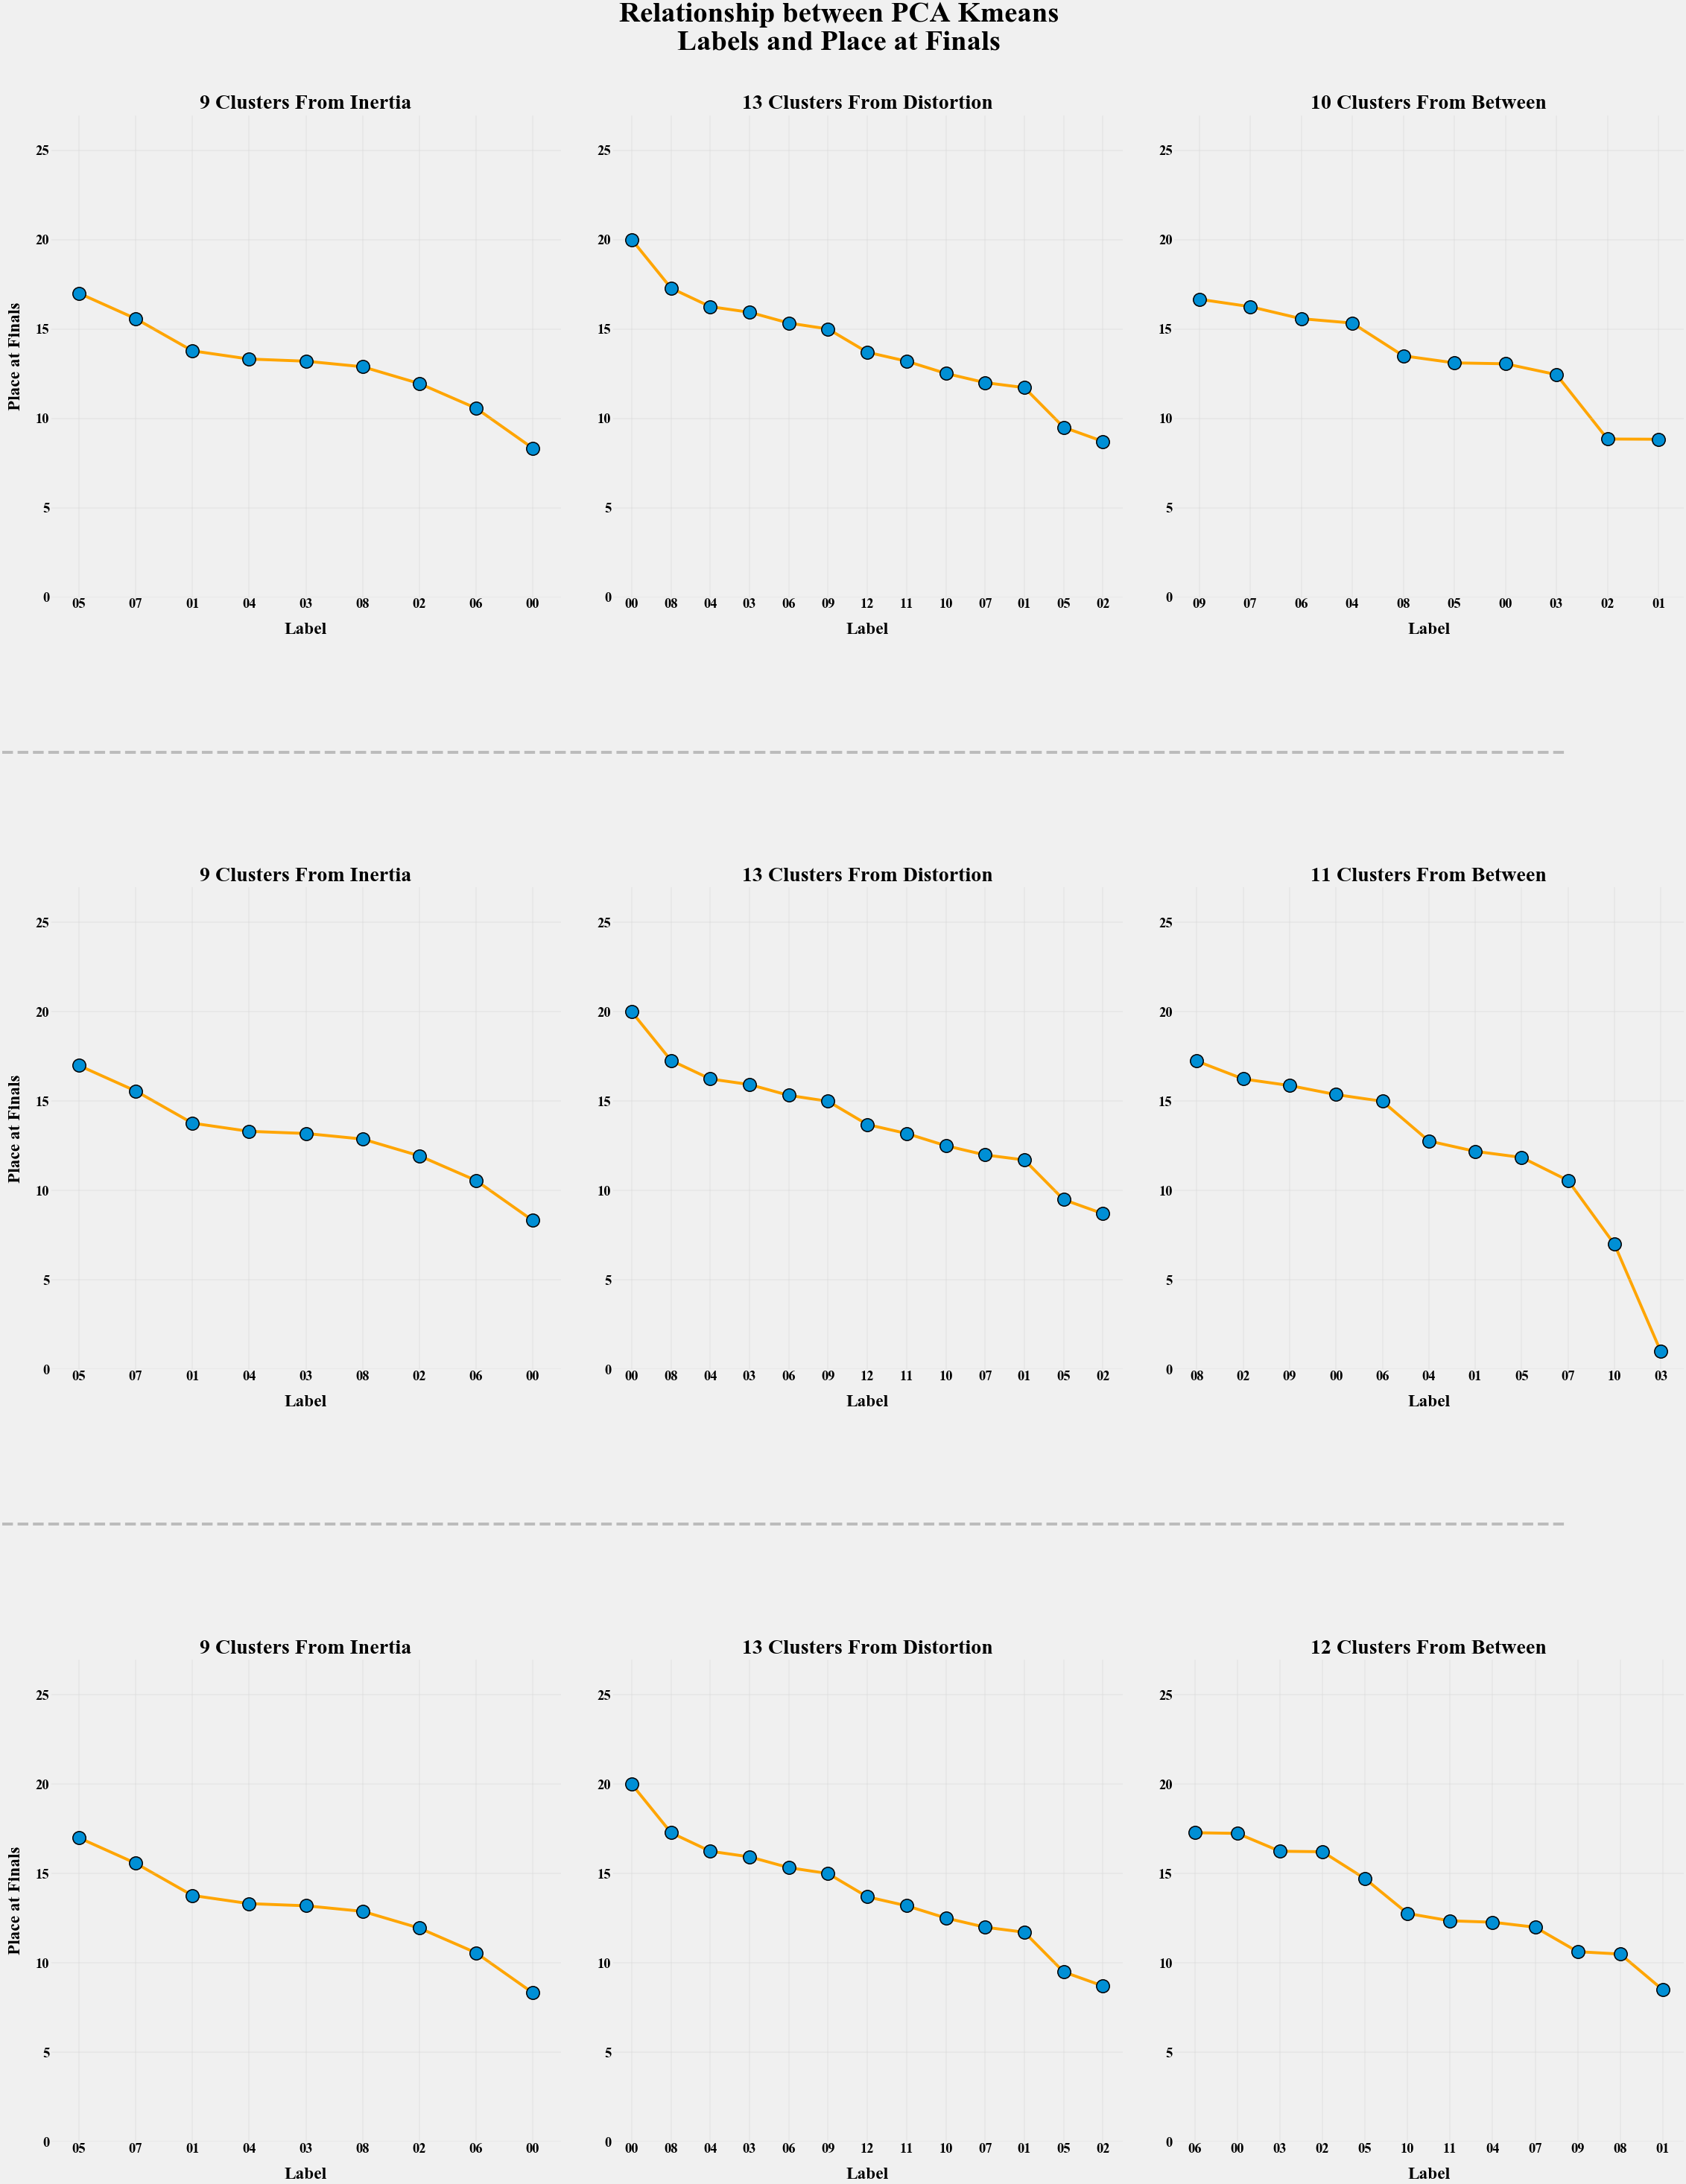
\includegraphics[width=\linewidth]{{final_plots/4_4_label_plot_pca_kmeans_inertia_distortion_between_10_11_12.png}}
  \centering
  \captionsetup{justification=centering}
  \caption{Plots of Clusters Against Average Place at the Finals to Evaluate Strength of Selection} 
  \label{fig:plot_kmeans_clusters}
\end{figure}

From \Cref{fig:plot_kmeans_clusters}

\begin{figure}[H]
  \includegraphics[width=\linewidth]{{final_plots/4_5_boxplot_pca_kmeans_9_10_11_12_13.png}}
  \centering
  \captionsetup{justification=centering}
  \caption{Boxplots of Varying Numbers of Clusters Against Place at Finals to Determine Optimal Number for Model} 
  \label{fig:boxplot}
\end{figure}

From \Cref{fig:boxplot}


% Discussion
\newpage
\section{Discussion}

\newpage
\section{References}
%\renewcommand\bibname{Name}
%\defbibheading{}{\section*{References}}
%\renewcommand\refname{}


%\bibliographystyle{APA}
%\bibliography{test.bib}
\nocite{*}
\printbibliography

%\bibliography{cap_bibliography.bib}
%\bibliography{cap_bibliography.bib}

\iffalse
\begingroup
\renewcommand{\section}[2]{}%
\renewcommand\bibindent{3em}
\setlength{\bibhang}{11pt}
\setlength{\bibitemsep}{6pt}
\begin{thebibliography}{99\kern\bibindent}
\bibitem{1}
  365 Data Science. (2020). How to combine PCA and K-Means in python?
  \textit{365 Data Science.}
  Retrieved from 365datascience.com/pca-k-means/.


\bibitem{2}
  Abakoumkin, G. (2018). Mere exposure effects in the real world: utilizing natural experiment 
  features from the eurovision song contest.
  \textit{}
  doi

\bibitem{3}
  
  \textit{}
  doi

\bibitem{4}
  
  \textit{}
  doi

\bibitem{5}
  
  \textit{}
  doi


\bibitem{6}
  
  \textit{}
  doi

\bibitem{7}
  
  \textit{}
  doi

\bibitem{8}
  
  \textit{}
  doi

\bibitem{9}
  
  \textit{}
  doi


\bibitem{10}
  
  \textit{}
  doi
  

\bibitem{11}
  
  \textit{}
  doi


\bibitem{12}
  
  \textit{}
  doi


\bibitem{13}
  
  \textit{}
  doi


\bibitem{14}
  
  \textit{}
  doi


\bibitem{15}
  
  \textit{}
  doi

\bibitem{16}
  
  \textit{}
  doi

\bibitem{17}
  
  \textit{}
  doi


\bibitem{18}
  
  \textit{}
  doi


\bibitem{19}
  
  \textit{}
  doi


\bibitem{20}
  
  \textit{}
  doi


\bibitem{21}
  
  \textit{}
  doi

\bibitem{22}
  
  \textit{}
  doi


\bibitem{23}
  
  \textit{}
  doi

\bibitem{24}
  
  \textit{}
  doi

\bibitem{25}
  
  \textit{}
  doi


\bibitem{26}
  
  \textit{}
  doi

\bibitem{27}
  
  \textit{}
  doi


\bibitem{28}
  
  \textit{}
  doi


\bibitem{29}
  
  \textit{}
  doi


\bibitem{30}
  
  \textit{}
  doi

\bibitem{31}
  
  \textit{}
  doi
  
\bibitem{32}
  
  \textit{}
  doi

\bibitem{33}
  
  \textit{}
  doi

\bibitem{34}
  
  \textit{}
  doi


\bibitem{35}
  
  \textit{}
  doi

\bibitem{36}
  
  \textit{}
  doi

\bibitem{37}
  
  \textit{}
  doi

\bibitem{38}
  
  \textit{}
  doi

\bibitem{39}
  
  \textit{}
  doi

\bibitem{40}
  
  \textit{}
  doi


\bibitem{41}
  
  \textit{}
  doi


\bibitem{42}
  
  \textit{}
  doi

\bibitem{43}
  
  \textit{}
  doi

\bibitem{44}
  
  \textit{}
  doi

\bibitem{45}
  
  \textit{}
  doi

\bibitem{46}
  
  \textit{}
  doi

\bibitem{47}
  
  \textit{}
  doi

\bibitem{48}
  
  \textit{}
  doi

\bibitem{49}
  
  \textit{}
  doi

\bibitem{50}
  
  \textit{}
  doi

\bibitem{51}
  
  \textit{}
  doi


\bibitem{52}
  
  \textit{}
  doi

\bibitem{54}
  
  \textit{}
  doi

  
\end{thebibliography}
\endgroup
\fi  
\end{document}

%%% Local Variables:
%%% mode: latex
%%% TeX-master: t
%%% End:
